%   This file is part of the APS files in the REVTeX 4.2 distribution.
%   Version 4.2a of REVTeX, December 2014
%
%   Copyright (c) 2014 The American Physical Society.
%
%   See the REVTeX 4 README file for restrictions and more information.
%
% TeX'ing this file requires that you have AMS-LaTeX 2.0 installed
% as well as the rest of the prerequisites for REVTeX 4.2
%
% See the REVTeX 4 README file
% It also requires running BibTeX. The commands are as follows:
%
%  1)  latex apssamp.tex
%  2)  bibtex apssamp
%  3)  latex apssamp.tex
%  4)  latex apssamp.tex
%
\documentclass[%
 reprint,
%superscriptaddress,
%groupedaddress,
%unsortedaddress,
%runinaddress,
%frontmatterverbose, 
%preprint,
%preprintnumbers,
%nofootinbib,
%nobibnotes,
%bibnotes,
 amsmath,amssymb,
 aps,
%pra,
%prb,
%rmp,
%prstab,
%prstper,
%floatfix,
]{revtex4-2}

\usepackage{graphicx}% Include figure files
\usepackage{dcolumn}% Align table columns on decimal point
\usepackage{bm}% bold math
\usepackage{float}
\usepackage{tikz}
\usepackage{pgfplots}
%\usepackage{enumitem}

%\usepackage{hyperref}% add hypertext capabilities
%\usepackage[mathlines]{lineno}% Enable numbering of text and display math
%\linenumbers\relax % Commence numbering lines

%\usepackage[showframe,%Uncomment any one of the following lines to test 
%%scale=0.7, marginratio={1:1, 2:3}, ignoreall,% default settings
%%text={7in,10in},centering,
%%margin=1.5in,
%%total={6.5in,8.75in}, top=1.2in, left=0.9in, includefoot,
%%height=10in,a5paper,hmargin={3cm,0.8in},
%]{geometry}

\begin{document}


\preprint{APS/123-QED}

\title{Combined and Composite Games in Evolutionary Game Theory}% Force line breaks with \\
\thanks{Submitted for MSci final year project report, computer science}%

\author{Henry Brooks}
\affiliation{%
 University of Birmingham
}%


\date{\today}% It is always \today, today,
             %  but any date may be explicitly specified

\begin{abstract}
The evolutionary dynamics of a composite four-strategy game formed by combining the cyclic Rock-Paper-Scissors (RPS)
game and the Snowdrift (SD) game, are investigated in infinite and finite populations. A payoff structure is
formed and cast into replicator equations, fixed points and stability of the four-strategy system are 
analyzed.

Finite population effects are studied under three different microscopic interaction processes:
the Moran process, the local update process, and the local fermi process. Analytical calculations
of drift observables and large ensemble agent based simulations are used to 
measure the stability of the system under different conditions and visualize the 
dynamics in the four-simplex.
Three drift observables $H_{\mathrm{SD}}$, $H_{\mathrm{RPS}}$, and $H_4$ are defined to 
characterise the stability of each subgame and for the full four-strategy game.

The main result demonstrates the phenomenon of drift reversal, a loss of stability below a critical population size, 
at two different critical population sizes $N^\prime_{\mathrm{RPS}}$ and 
$N^\prime_{\mathrm{SD}}$ for each of the subgames. For the local update process a closed form expression for 
both $N^\prime_{\mathrm{RPS}}$ and $N^\prime_{\mathrm{SD}}$ are derived.
The ordering of $N^\prime_{\mathrm{RPS}}$ and $N^\prime_{\mathrm{SD}}$ result in qualitatively different
dynamics and four main cases are visualized in the four-simplex of the game: 
a disk-like cloud in the RPS plane, a column-shaped cloud in the Snowdrift axis, full interior coexistence in the large 
population case, and a double drift reversal at very small population sizes $N << N^\prime_{\mathrm{RPS}}, 
N << N^\prime_{\mathrm{SD}}$ where trajectories are absorbed by the boundaries. 
\end{abstract}

%\keywords{Suggested keywords}%Use showkeys class option if keyword
                              %display desired
\maketitle

%\tableofcontents

\section{\label{sec:level1}Introduction}


Evolutionary game theory provides a framework for analyzing the dynamics of 
competing strategies in biological and social systems ranging from animal behaviour \cite{rps_lizard} and
microbial interactions \cite{cheating_microbes,yeast_snowdrift} to economics.
Replicator equations \cite{evolution_pop_dynamics,evolution_maynard} describing the 
time evolution of strategy frequencies in a population can be formed under frequency dependent selection 
and the comparison of individual fitness from a payoff structure. The Rock-Paper-Scissors game (RPS)
is used as a model for cyclic dominance with famous biological examples including the 
dynamics of the side-blotched lizard populations \cite{rps_lizard} and competition in strains of E.coli \cite{rps_ecoli}.
The Snowdrift game (SD) models a tradeoff between cooperation and defection when some negative cost is shared between 
the players resulting in a mixed strategy Nash equilibrium \cite{evolution_maynard} with biological examples including 
the production of the enzyme invertase in yeast cells \cite{yeast_snowdrift}. 

In this project I explore the evolutionary dynamics of a four-strategy
game composed of the two-strategy SD game and the three-strategy RPS game 
to form a combined game with the payoff matrix (equation~\ref{AugRpsMatrix}).
The composite game combines the cyclic dominance with cooperation/defection coexistence dynamics
with invasion into the RPS cycle by the SD strategy. A game of this form has been considered 
in the infinite-population case \cite{evolution_pop_dynamics}, this project extends this analysis to the 
finite populations, focusing on the phenomenon of drift reversal~\cite{drift_reversal_paper}.

In finite populations noise is introduced into the dynamics that has been shown 
to qualitatively alter the dynamics of a game described 
by replicator equations \cite{drift_reversal_paper,Claussen2007-zo,rps_cyclic_jens,general_moran_process}.
Drift reversal occurs when an attracting fixed point loses stability below a critical population size, 
and this depends on the initial parameters of the game, the strength of selection and the underlying
microscopic update process \cite{drift_reversal_paper}. This has been analyzed for 
two-strategy games and the three-strategy RPS game in Refs.~\cite{rps_cyclic_jens,drift_reversal_paper}.
This project demonstrates that in the composite RPS-SD game there are two independent critical population sizes
for a drift reversal in each of the subgames and that the relative ordering of these two population sizes 
result in distinct dynamics illustrated in section~\ref{sec:drift_measures}.

This report first introduces the RPS and SD game individually in sections \ref{RPS-model} and \ref{SD-model}. 
Section \ref{sec:combined_game} introduces the payoff structure and stability analysis for the combined game 
in the infinite population case. Section \ref{sec:interaction_processes} discusses the three microscopic 
interaction processes and 
defines transition probabilites for individuals hopping from one strategy to another. Section 
\ref{sec:fokker-planck} and \ref{sec:drift_measures} derive a 
Fokker-Planck equation and drift measures to quantify the stochastic effects of finite populations and 
calculate the critical population sizes where drift reversal occurs. A closed form solution for the local update process
critical population size is derived, and finally the distinct drift reversal cases are compared.

A simulation library has been developed alongside this report. This implements agent based simulations for the three
update processes, numerical integration of the replicator equations derived from the 
Fokker-Planck expansion, and numerical computation of the drift observables. It also contains 
visualization tools for the trajectories for $2 \times 2, 3 \times 3, 4 \times 4$ games in finite and infinite 
populations. Full source code and usage instructions are available in the project repository~\cite{project_appendix}.

\subsection{\label{RPS-model} Rock-Paper-Scissors}
The general RPS payoff matrix is defined as:
\begin{align}
\begin{bmatrix}
    a & c & b\\
    b & a & c\\
    c & b & a
\end{bmatrix}
\end{align}
For the standard symmetric case of the RPS game, $a = 0, c = -1, b = 1$.
Here rock crushes scissors, paper covers rock, and scissors cuts paper. 
Ties are awarded the payoff of 0, resulting in cyclic dynamics about the internal
fixed point of $\left(\frac{1}{3}, \frac{1}{3}, \frac{1}{3}\right)$.

\subsubsection{\label{sec:rps_replicator} Replicator dynamics}

To analyze the time evolution of a population under the RPS game, 
the standard imitation-based replicator equations are derived for the system.
Let $x$, $y$ and $z$ represent the fraction of players using rock, paper, and scissors
respectively. The fraction of scissors players $z$ can be defined as $z = 1 - x - y$, 
reducing the dimension of the replicator equations.
Expected payoffs for each strategy can then be defined as follows:
\begin{align}
   \pi_R &= a x + b \left(1- x - y\right) + c y \nonumber \\
   \pi_P &= a y + b x + c \left(1- x - y\right) \nonumber\\
   \pi_S &= a \left(1-x-y\right) + b y + c x \nonumber
\end{align}

Using the standard replicator model for the evolution of population fractions over time, where
the payoff of a strategy is compared to the average payoff, the 
following equation \cite{evolution_pop_dynamics} can be used to define a series of differential equations for 
each of the population fractions:

\begin{equation} \label{eq:standard_replicator_dynamics}
\dot x_i = x_i(\pi_i(x) - \langle \pi(x) \rangle)
\end{equation}

where the average payoff is:
\begin{equation}
\langle \pi(x) \rangle = x \pi_R + y \pi_P + z \pi_S
\end{equation}


This leads to the two differential equations for the evolution of the population fractions $x$ and $y$ 
over time:

\begin{widetext}
\begin{equation}
    \begin{split}
        \dot{x} &= x y \left(a x - a y - b x + b \left(-x - y + 1\right) + c y 
        - c \left(-x - y + 1\right)\right) \\
        & + x \left(-x - y + 1\right) \left(a x - a \left(-x - y + 1\right)
        - b y + b \left(-x - y + 1\right) - c x + c y\right)
    \end{split}
\end{equation}
\begin{equation}
    \begin{split}
        \dot{y} &= x y \left(- a x + a y + b x - b \left(- x - y + 1\right) - c y 
        + c \left(- x - y + 1\right)\right) \\
        & + y \left(- x - y + 1\right) \left(a y - a \left(- x - y + 1\right)
        + b x - b y - c x + c \left(- x - y + 1\right)\right)
    \end{split}
\end{equation}
\end{widetext}
The fraction of $z$ players can be found with $z = 1-x-y$.

These are the deterministic replicator equations from 
evolutionary game theory which define populations $x,y,z$ over time. These are extended in section \ref{sec:fokker-planck}
for specific microscopic interaction processes including the noise terms that appear
due to the finite population size effects.

The stability of this system of replicator equations can be analyzed by
computing the eigenvalues of the Jacobian of the replicator system, following standard
methods in evolutionary game theory \cite{evolution_pop_dynamics}:

\begin{equation}
J = 
\begin{bmatrix}
\frac{\partial F}{\partial x} & \frac{\partial F}{\partial y} \\
\frac{\partial G}{\partial x} & \frac{\partial G}{\partial y}
\end{bmatrix}
\end{equation}
where $F = \dot x, G = \dot y$.
Full expansions of $\frac{\partial F}{\partial x},
\frac{\partial F}{\partial y},\frac{\partial G}{\partial x}, \frac{\partial G}{\partial y} $
are provided in the appendix.

Fixed point stability can be determined by computing the eigenvalues of this matrix $J$ at 
a specific point.

For the standard RPS game where $a = 0, b = 1, c = -1$ the eigenvalues of the RPS game are:

\begin{align}
\lambda_1 &= -\frac{1}{2} \sqrt{16 x^{2} + 16 x y - 16 x + 16 y^{2} - 16 y + 4} \\
\lambda_2 &= \frac{1}{2} \sqrt{16 x^{2} + 16 x y - 16 x + 16 y^{2} - 16 y + 4}
\end{align}
and at the internal fixed point of $\left(\frac{1}{3}, \frac{1}{3}\right)$ for RPS, this gives:
\begin{align}
\lambda_1, \lambda_2 = \left\{- \frac{\sqrt{3}}{3} i, \frac{\sqrt{3}}{3} i\right\}
\end{align}
Since $\operatorname{Re}(\lambda_{1,2}) = 0$ and the eigenvalues are purely imaginary,
the interior fixed point is a nonlinear center and the trajectories form closed periodic 
orbits at a fixed distance determined by the initial population fractions as seen in 
Fig.~\ref{fig:rps_standard}.


\begin{figure}
\centering
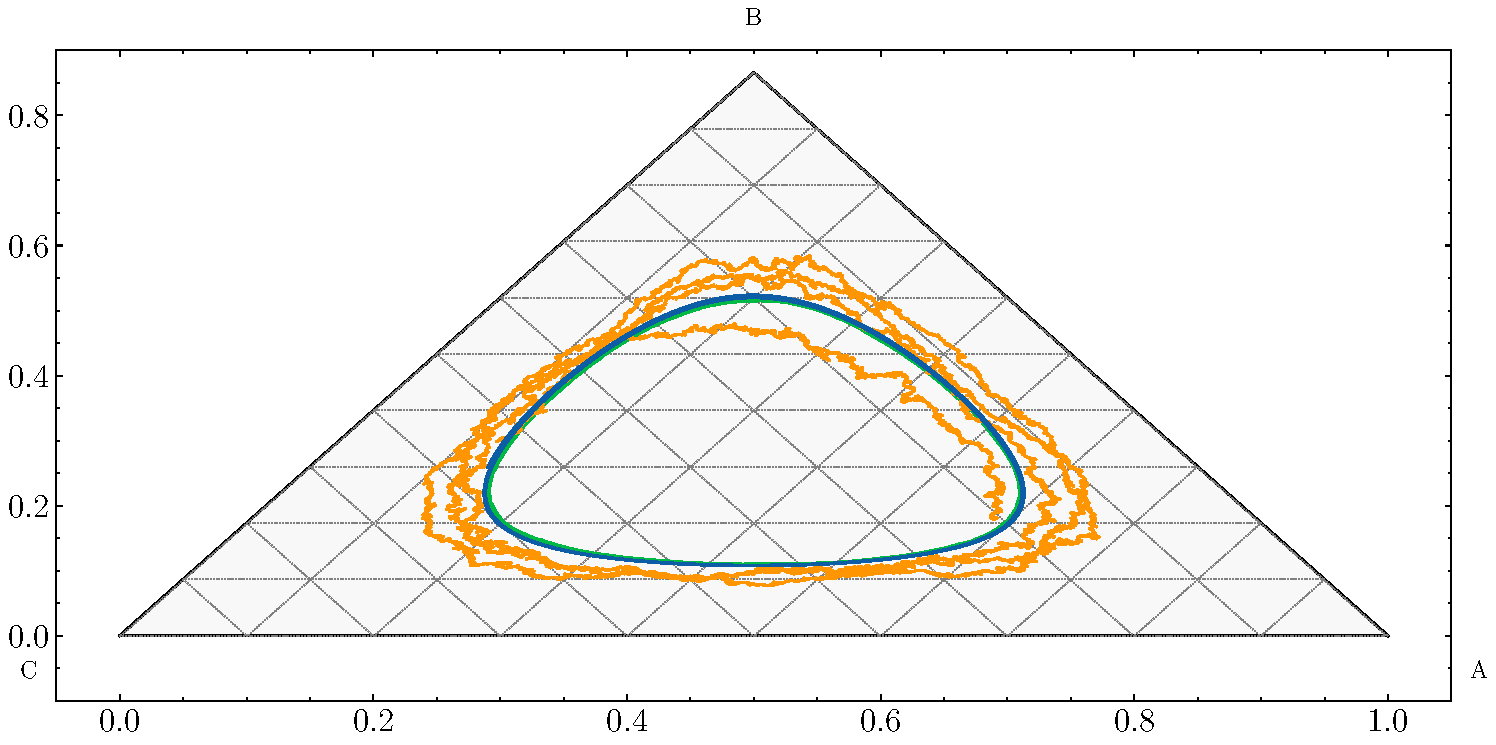
\includegraphics[scale=0.3]{Figures/rps_standard.pdf}
\caption{\label{fig:rps_standard} Standard zero sum RPS game. $w = 0.3$, analytical trajectory (blue), 
large $N$ (500000) in green and small $N$ (2000) in orange for comparison. Large $N$ closely follows
the replicator dynamics as expected, small $N$ is heavily influenced by noise
and doesn't precisely follow dynamics. Agrees with stability analysis, periodic 
orbits at a fixed distance determined by the initial population.}
\end{figure}



In the rest of this report I will focus on the case where $a = 0, b = 1$ and $c$ is left as a free parameter which 
governs the dynamics of the game. In the standard zero-sum case where $c=-1$, the system is neutrally stable and the 
trajectories oscillate at a fixed distance from the Nash equilibrium $(1/3, 1/3, 1/3)$. 
When $c < -1$ the system spirals outwards from the equilibrium and will be absorbed by the boundaries and
finally when $c > -1$ the system will spiral inwards, where cooperation between the three strategies is
preferred. It has previously been shown that a drift reversal effect occurs when $c > -1$ where a critical 
population size can reverse the drift from the internal stable point towards the boundaries \cite{rps_cyclic_jens}.

\begin{figure} 
\centering
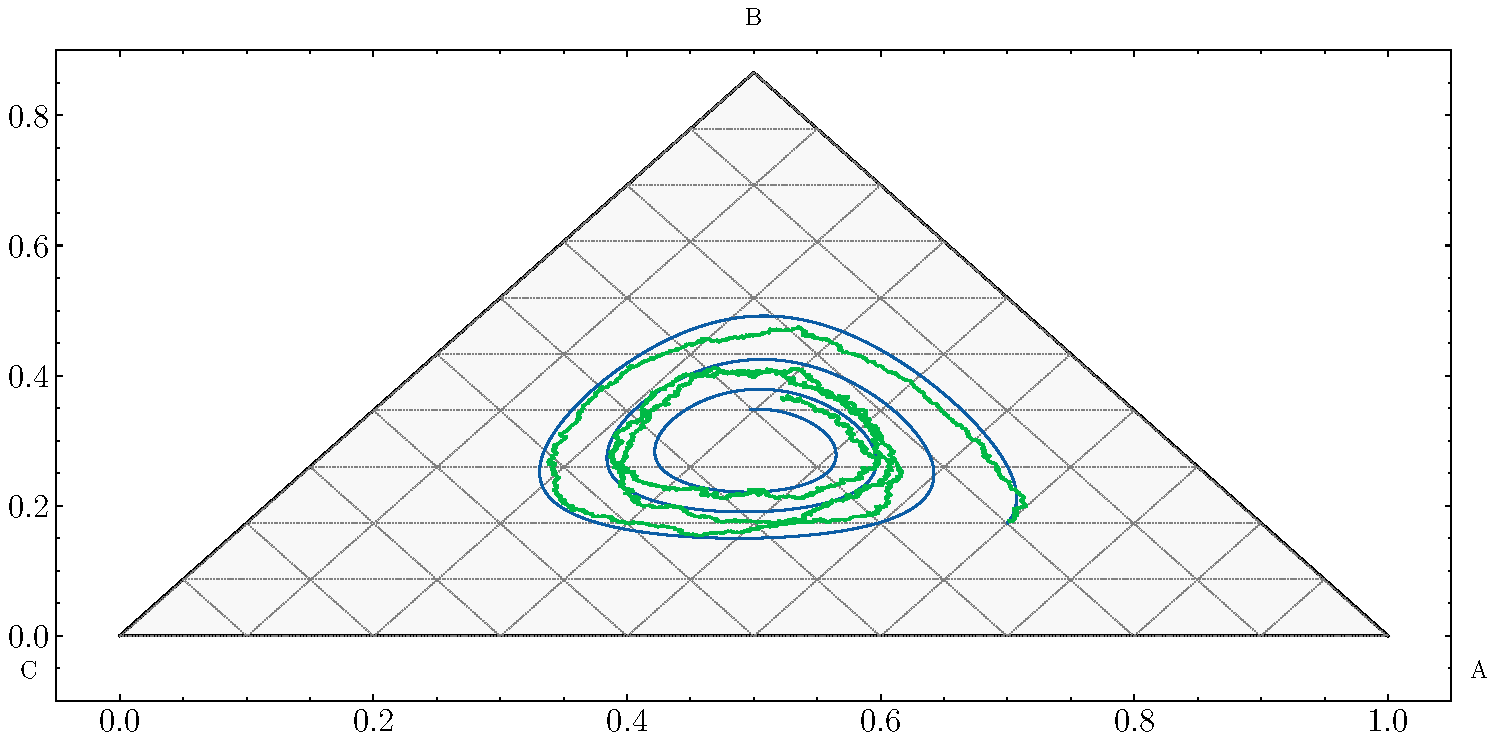
\includegraphics[scale=0.3]{Figures/rps_example_in_spiral.pdf}
\caption{\label{fig:rps_sink} Trajectory for the RPS game where $c = -0.8$. The blue line corresponds to a numerical
solution of the adjusted replicator dynamics for the Moran process, and the green line is a Moran process
agent based simulation with a population size of 500. Strength of selection $w = 0.3$.
With a population size of 500, the agent based simulation follows the deterministic trajectory rather well,
with deviations from the deterministic trajectory due to stochastic fluctuations caused by the finite population size.}
\end{figure}


The eigenvalues of the game in Fig.~\ref{fig:rps_sink} are:
\begin{equation}
\lambda_{1}, \lambda_2 = \left\{-\frac{1}{30} + \frac{3 \sqrt{3}}{10}i,
-\frac{1}{30} - \frac{3 \sqrt{3}}{10}i\right\}
\end{equation}
Since the real parts of the eigenvalues are negative, 
$\operatorname{Re}(\lambda_{1,2}) = -\frac{1}{30} < 0$, the fixed point $\left(\frac{1}{3}, \frac{1}{3}\right)$
is linearly stable, so the populations will converge towards the central fixed point over time.
The imaginary component indicates the oscillatory dynamics so the population will spiral inwards 
towards the center. When $c = -0.8$, the populations converge towards a stable
coexistence. For this particular case of RPS a drift reversal can occur in finite populations 
\cite{rps_cyclic_jens}.

\subsection{\label{SD-model} Snowdrift}

The snowdrift game has also been intensely 
studied \cite{evolution_maynard} 
and is an example of an anti-coordination where there are two pure strategy Nash equlibria when 
players select opposite strategies.
The game is defined by the following payoff matrix with rows corresponding to 
cooperation and defection.

\begin{align}
\begin{bmatrix}
    (\frac{b}{2}-\frac{c}{2}, \frac{b}{2}-\frac{c}{2}) & (\frac{b}{2}-c,\frac{b}{2}) \\ \\
    (\frac{b}{2}, \frac{b}{2} - c) & (0,0)
\end{bmatrix}
\end{align}

The snowdrift game describes a scenario of two drivers trapped in a snowdrift.
They have the options to shovel the snow and clear a path (cooperate) or stay in their car (defect).
If both cooperate then they pay a shared cost $\frac{c}{2}$ but share the full benefit and can 
both drive. However the best outcome for one player is to remain in their car and let the other do
all the work in turn leaving the full cost $c$ to the other player but if both players
remain in their car then both remain stranded and receive a payoff of 0. This scenario 
often arises in biology and social/economic settings where mutual cooperation would be 
beneficial and both parties refusing to yield results in the worst outcome.

There are two pure strategy Nash equilbria where the players select opposite strategies, 
and a mixed strategy Nash equilibrum.
The interior mixed strategy Nash equilbrium for this payoff matrix occurs at the mixed strategy $q^* = \frac{b-2c}{b-c}$ where 
$q$ denotes the fraction of cooperators.

In the example trajectory where $b=3, c=1$, the mixed strategy evaluates to 
being $(\frac{1}{2},\frac{1}{2})$, and is a stable fixed point in the system as seen in 
Fig.~\ref{snowdrift_trajectory}.

\begin{figure}
\centering
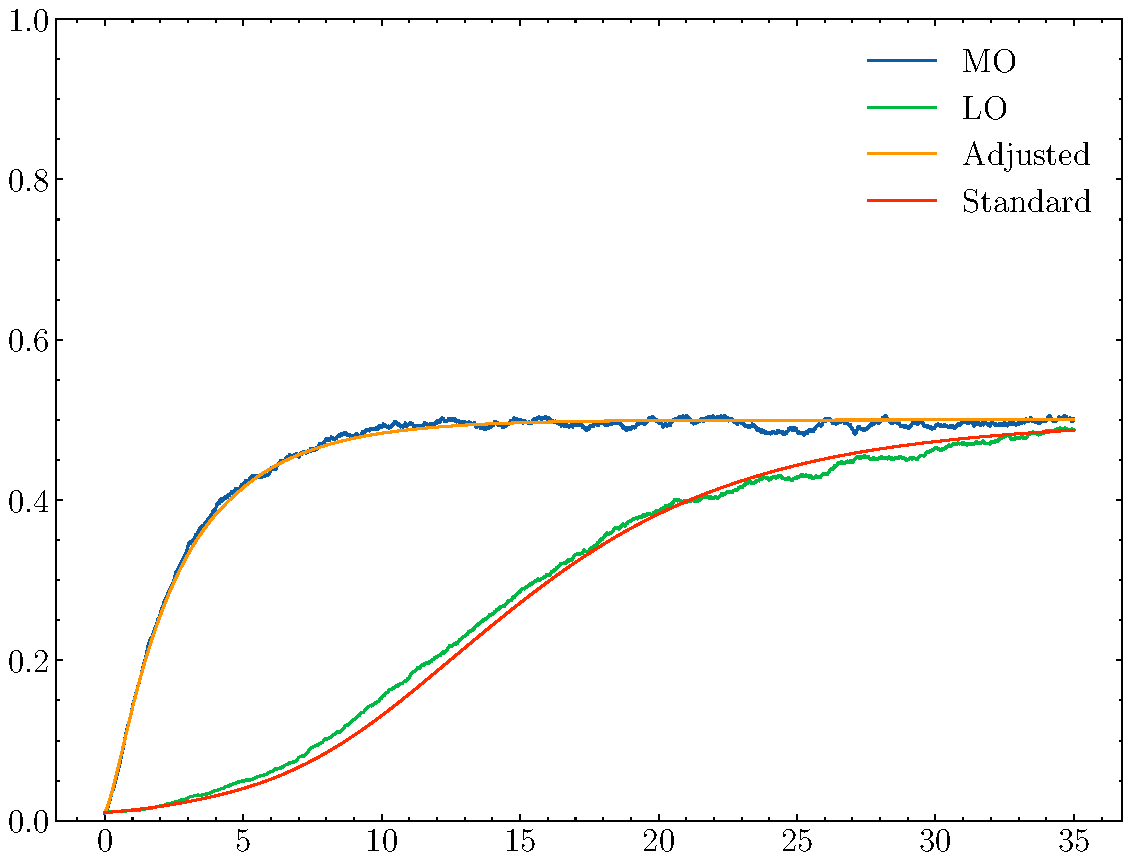
\includegraphics[scale=0.4]{Figures/snowdrift_sim.pdf}
\caption{\label{snowdrift_trajectory}Snowdrift game population time series for Local update (LU) and Moran process (MO), 
alongside solution to deterministic replicator equation for each process from the 
adjusted dynamics derived in section.~\ref{sec:fokker-planck}. $N = 10000$, large population size trajectories 
closely follow deterministic path. $w=0.9$, initial population 99\% cooperators. The game
fixes at the mixed strategy Nash equilibrium $(\frac{1}{2}, \frac{1}{2})$}
\end{figure}


\section{\label{sec:combined_game}Combined game definition}

The focus of this work is a composite game formed by combining
the snowdrift (SD) and rock-paper-scissors (RPS) games
into a single four-strategy payoff matrix. Average payoffs, 
replicator equations and fixed points can 
subsequently be derived and the deterministic dynamics can be studied.

These dynamics have been considered before \cite{evolution_pop_dynamics}, 
however not in extensive detail nor in finite populations. 
The remainder of this report demonstrates that there 
is a drift reversal and that this occurs at different population sizes, 
and can be tuned to provide different distinct cases, 
resulting in qualitatively different dynamics from the infinite/large 
population case depending on the relative critical population sizes of the sub games. 


The combined game is defined as:

\begin{align}
\label{AugRpsMatrix}
\mathbf{A} =
\begin{bmatrix}
    a & c & b & \gamma\\
    b & a & c & \gamma\\
    c & b & a & \gamma\\
    a + \beta & a + \beta & a + \beta & 0
\end{bmatrix}
\end{align}
where the values $a,b,c$ represent the RPS cyclic game.

When $a = 0$, standard RPS ties, this can be reduced to the $2 \times 2$ snowdrift context as the following
payoff matrix:
\begin{align} \nonumber
\label{CompositeGame}
\begin{bmatrix}
    \langle RPS \rangle & \gamma\\
    \beta & 0 \\
\end{bmatrix}
\end{align}
Where $\langle RPS \rangle$ is the expected value of the RPS game.
The drift observable $H_{SD}$ (equation \ref{eq:delta_h_sd}) will measure the distance
from the fixed point of this game purely in the SD context (the vertical column in the 
four-simplex).

The population can be visualized as a 3d projection of a four-simplex 
with each of the RPS strategies being in the bottom three corners forming an 
RPS plane, and the fourth strategy being at the top forming a SD vertical axis.
If there are no players in the fourth strategy, then this collapses to the 
same RPS dynamics discussed previously.

\subsection{Replicator dynamics}

The payoffs for this game are:

\begin{align}
    \pi_R &= a x + b z + c y + \gamma (1 - x - y - z) \nonumber \\
    \pi_P &= a y + b x + c z + \gamma (1 - x - y - z) \nonumber \\
    \pi_S &= a z + b y + c x + \gamma (1- x - y - z)\nonumber  \\
    \pi_+ &= x (a + \beta) + y (a + \beta) + z (a + \beta)\nonumber 
\end{align}
Using $+$ to denote the 4th strategy.

The standard replicator dynamics \cite{evolution_pop_dynamics} (equation \ref{eq:standard_replicator_dynamics}) 
considering the case where $N$ is infinitely large are:

\begin{widetext}
\begin{align} 
\dot x &= x (a x + b z + c y + \gamma (1- x - y - z) - x (a x + b z + c y 
+ \gamma (1- x - y - z ))  - y (a y + b x + c z + \gamma (1- x - y - z))  \nonumber\\ 
&- z (a z + b y + c x 
+ \gamma (1- x - y - z))  - (x (a + \beta) + y (a + \beta) + z (a + \beta)) (1- x - y - z)) \nonumber
\end{align}
\begin{align}
\dot{y} &= y \big(a y + b x + c z + \gamma (1-x - y - z)
- x (a x + b z + c y + \gamma (1-x - y - z ))  - y (a y + b x + c z + \gamma (1-x - y - z)) \nonumber\\
&- z (a z + b y + c x + \gamma (1-x - y - z))  - (x (a + \beta) + y (a + \beta) + z (a + \beta)) (1-x - y - z) \big) \nonumber
\end{align}
\begin{align}
\dot{z} &= z \big(a z + b y + c x + \gamma (1-x - y - z)
- x (a x + b z + c y + \gamma (1-x - y - z)) - y (a y + b x + c z + \gamma (1-x - y - z )) \nonumber\\
&- z (a z + b y + c x + \gamma (1-x - y - z)) - (x (a + \beta) + y (a + \beta) + z (a + \beta)) (1-x - y - z) \big) \nonumber
\end{align}
\end{widetext}



Defining $F = \dot{x}, G = \dot{y}, P = \dot{z}$ the Jacobian for this system is:

\begin{equation}
J = 
\begin{bmatrix}
\frac{\partial F}{\partial x} & \frac{\partial F}{\partial y} &\frac{\partial F}{\partial z} \\[6pt]
\frac{\partial G}{\partial x} & \frac{\partial G}{\partial y} &\frac{\partial G}{\partial z} \\[6pt]
\frac{\partial P}{\partial x} & \frac{\partial P}{\partial y} & \frac{\partial P}{\partial z}
\end{bmatrix}
\end{equation}


Considering one particular instance of this game where
$a = 0, b=1, c= -1$ (standard rock paper scissors) and $\gamma = 0.2, \beta = 0.1$, 
there is an internal fixed point at $\left(\frac{2}{9},\frac{2}{9},\frac{2}{9},\frac{1}{3}\right)$.
The eigenvalues of this system are:

\begin{align}
\lambda_1, \lambda_2, \lambda_3 = \left\{-\frac{1}{15}, 
\frac{2\sqrt{3}}{9}i, -\frac{2\sqrt{3}}{9}i
\right\} \nonumber\\
\end{align}

The negative real eigenvalue here $-\frac{1}{15}$ indicates the 
stable plane where the trajectories will converge to (the snowdrift direction), and 
the pair of purely imaginary eigenvalues indicate the nonlinear center as 
before for stanrd rock paper scissors seen in Fig.~\ref{fig:rps_standard}.
This means the system will converge to the fixed points RPS plane, and then 
oscillate at a fixed distance from the center point
 $\left(\frac{2}{9},\frac{2}{9},\frac{2}{9},\frac{1}{3}\right)$. See the solved trajectory 
 against simulated fininte population trajectory in Fig.~\ref{fig:arps_standard_simplex} and 
 Fig.~\ref{fig:arps_standard_time_series} for the normalized time series. Normalization is done for simulated 
 results where simulated iterations are divided by the population size to match the time steps for 
 the solved differential equations in this case 150 time steps which was sufficient to show the fixation at the 
 stable orbit in the plane of the fixed point.


\begin{figure}
\centering
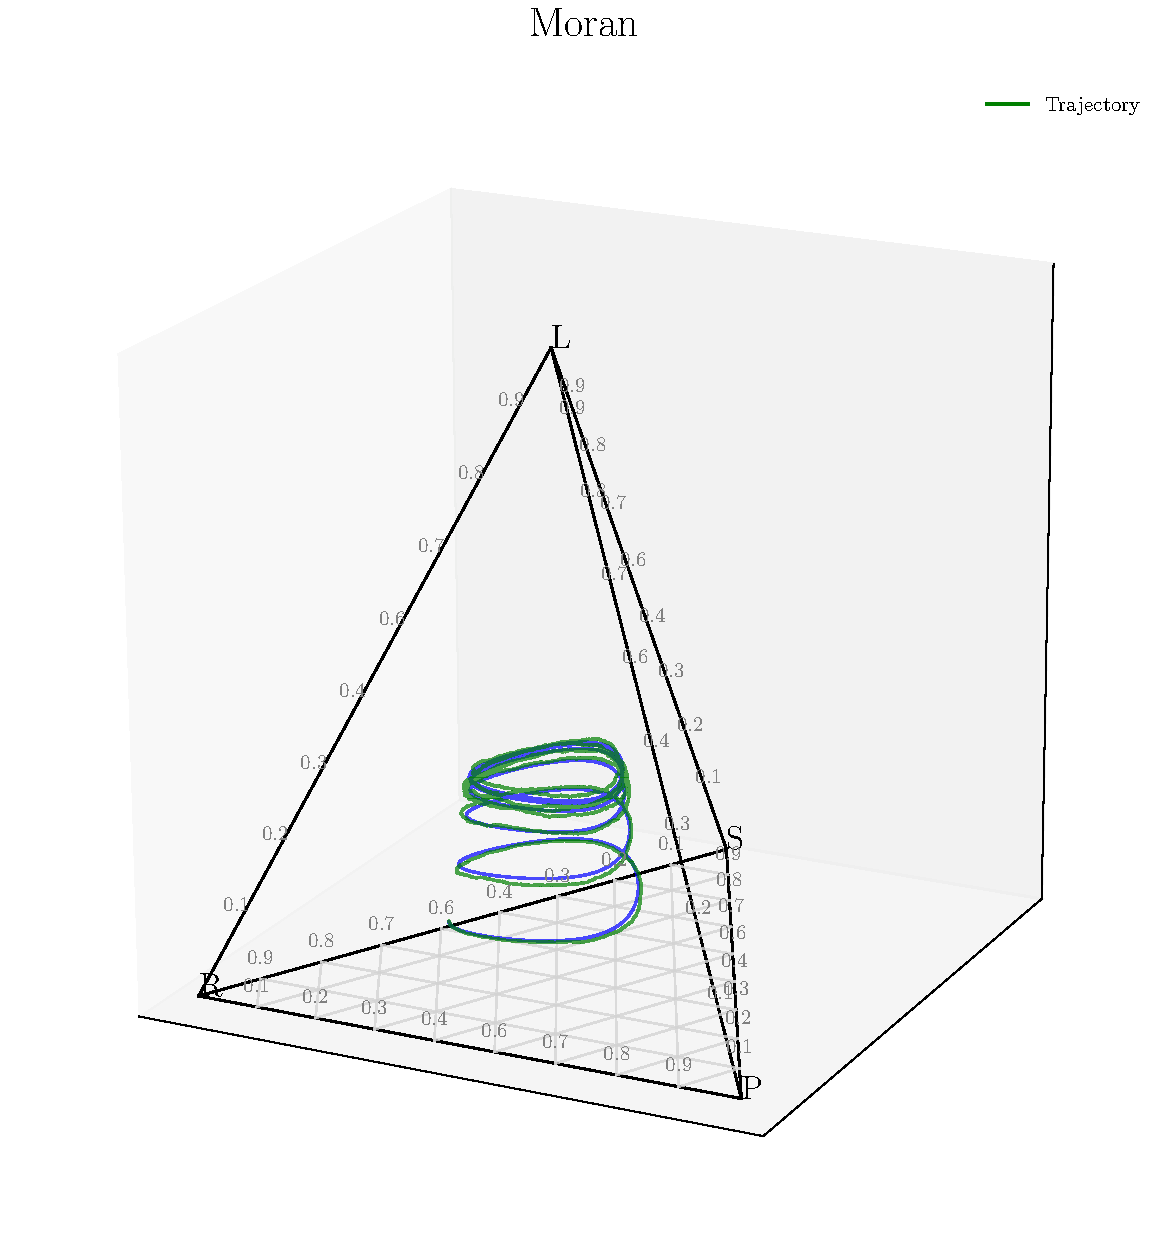
\includegraphics[scale=0.43]{Figures/arps_standard_simplex.pdf}
\caption{\label{fig:arps_standard_simplex} Simplex trajectory, numerical / sim, 
w = 0.45, N = 50000, 150 time steps - normalized iterations N * 150 for simulation
initial population [0.5,0.2,0.2, 0.1], RPS+, Standard RPS case
corresponding to eigenvalues shown before $\gamma=0.2, \beta=0.1$, shows
convergence to plane then periodic orbits at fixed distance from
center (2/9, 2/9,2/9,1/3)}

\end{figure}

\begin{figure*}
\centering
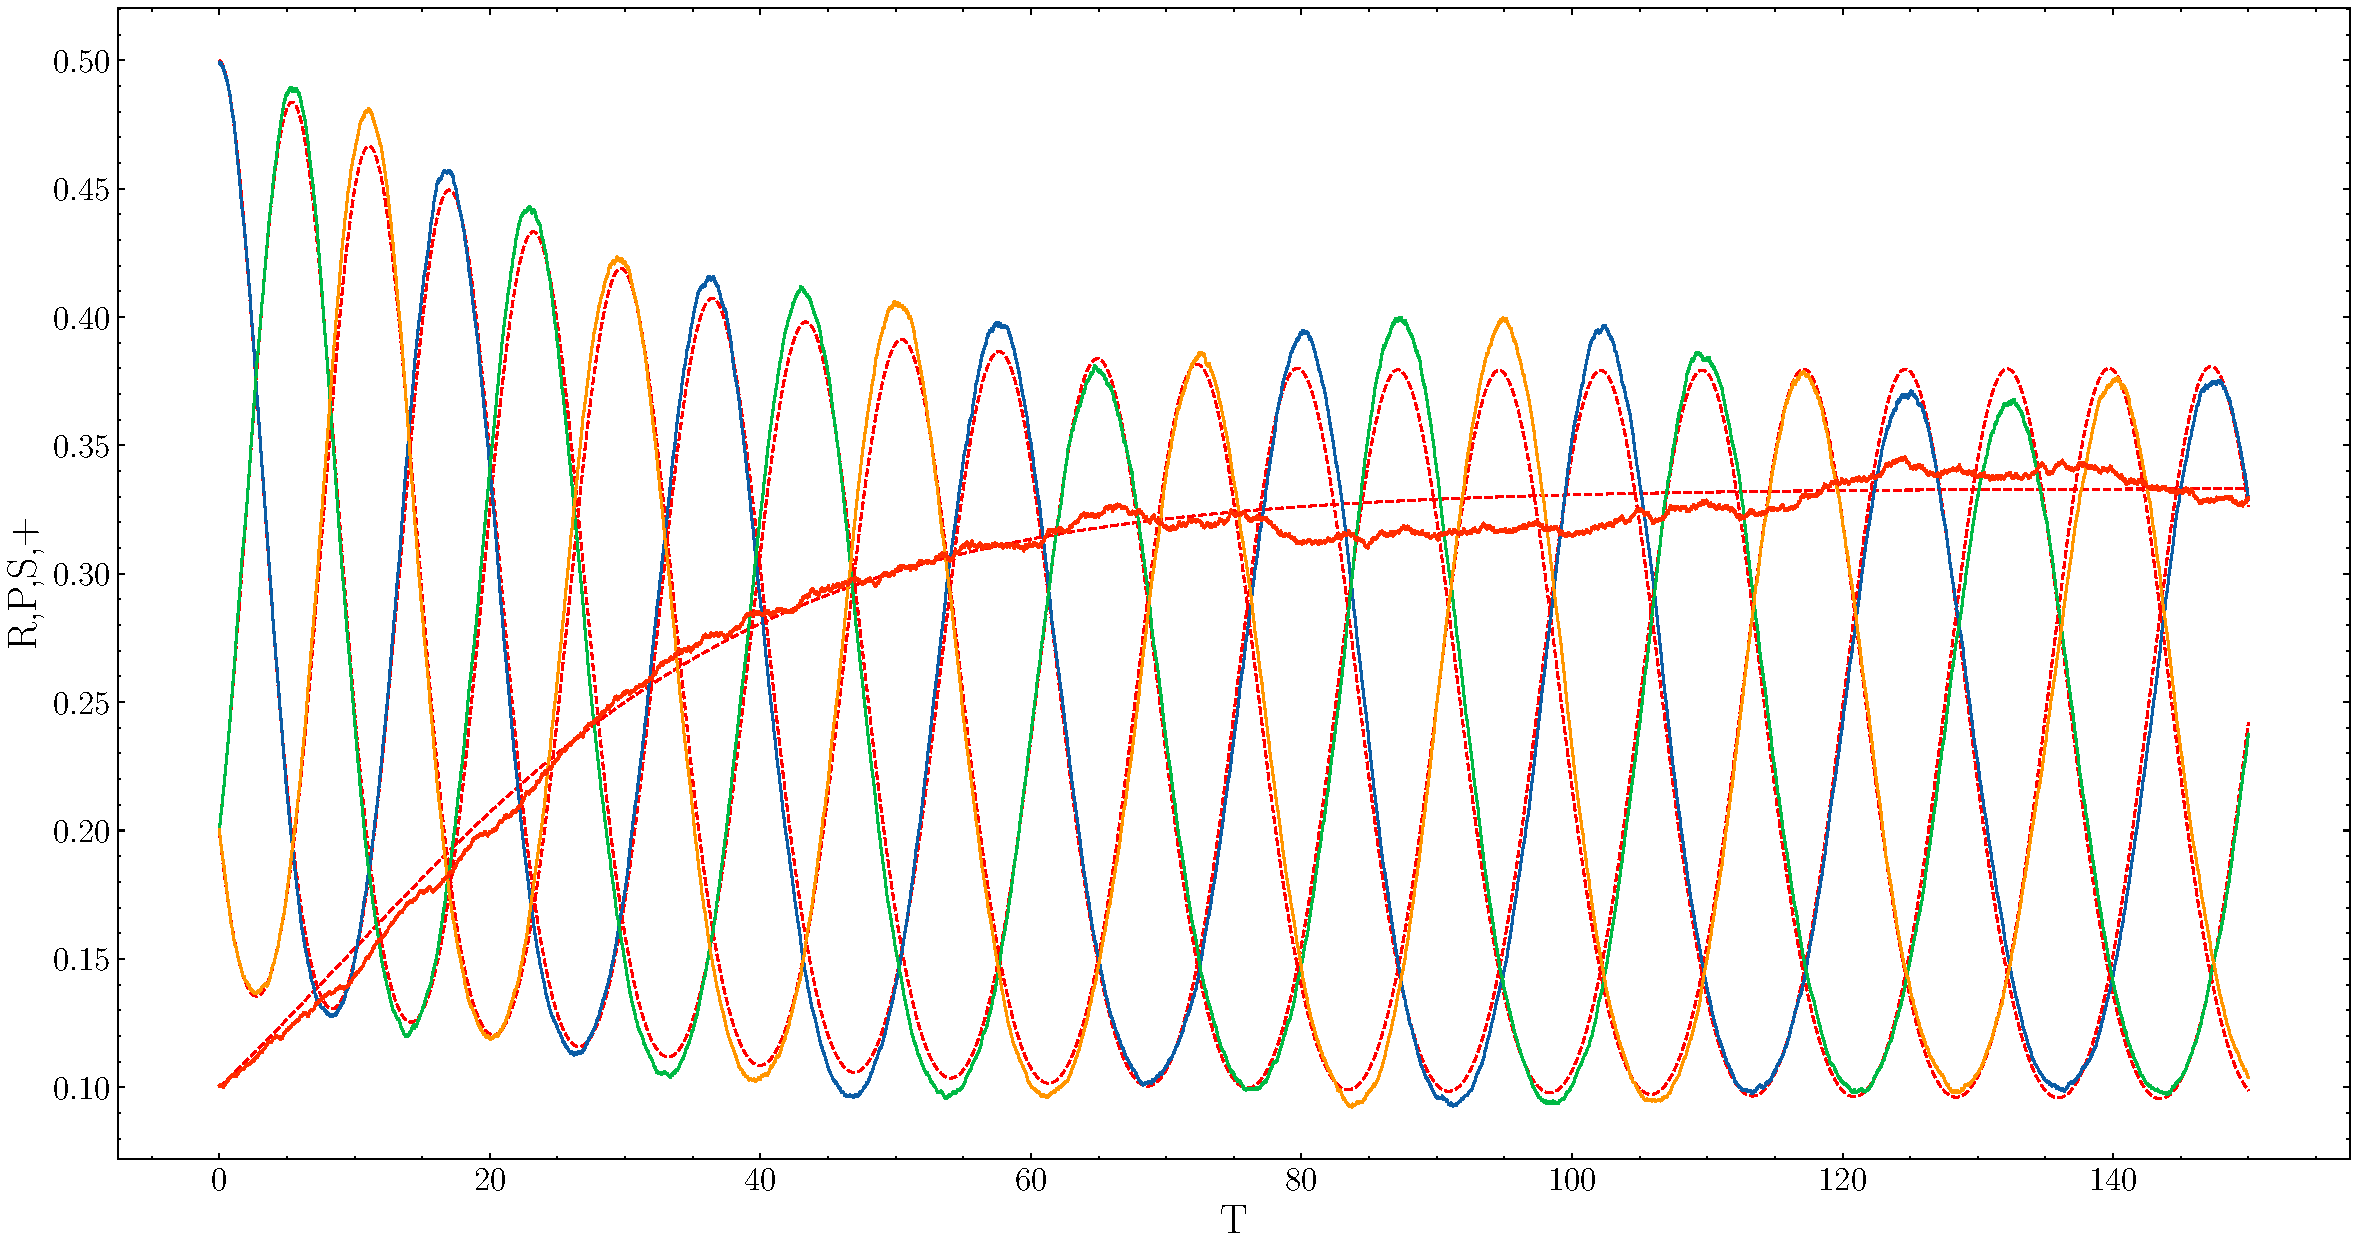
\includegraphics[scale=0.4]{Figures/arps_time_series_standard.pdf}
\caption{\label{fig:arps_standard_time_series} Time series, for the same data plotted in 
Fig.~\ref{fig:arps_standard_simplex}, dashed line corresponds to the solved system of ODE's from the 
Moran adjusted dynamics, $a(x)$ from the Fokker-planck derivation.}
\end{figure*}

As for RPS, setting parameter $c = -0.8$ or any $c > -1$, the RPS system becomes
attracting and the system would converge to the fixed points RPS plane,
whilst also being attracted inwards to the fixed point indicating a stable 
coexistence of all four strategies. In this case the interior four strategy coexistence fixed point is 
$\left( \frac{2}{7},\frac{2}{7},\frac{2}{7}, \frac{1}{7} \right)$.
The eigenvalues in this case ($c=-0.8$) are:

\begin{align}
\lambda_1, \lambda_2, \lambda_3 = \left\{-\frac{1}{35}, 
-\frac{1}{35} + \frac{9\sqrt{3}}{35}i, -\frac{1}{35} - \frac{9\sqrt{3}}{35}i
\right\} \nonumber\\
\end{align}
these eigenvalues describe the dynamics in Figs.~\ref{fig:arps_spiral_in}-\ref{fig:arps_spiral_in_time_series}, similarly to the neutral cycles
case where the first negative real eigenvalue describes convergence to the stable 
fixed point in the SD axis of the simplex. The eigenvalues 2 and 3 both contain negative real components 
indicating a stable attracting fixed point in the RPS plane (spirals inwards towards fixed point), and the imaginary 
components once again indicate the oscillatory nature of these trajectories.


\begin{figure}
\centering
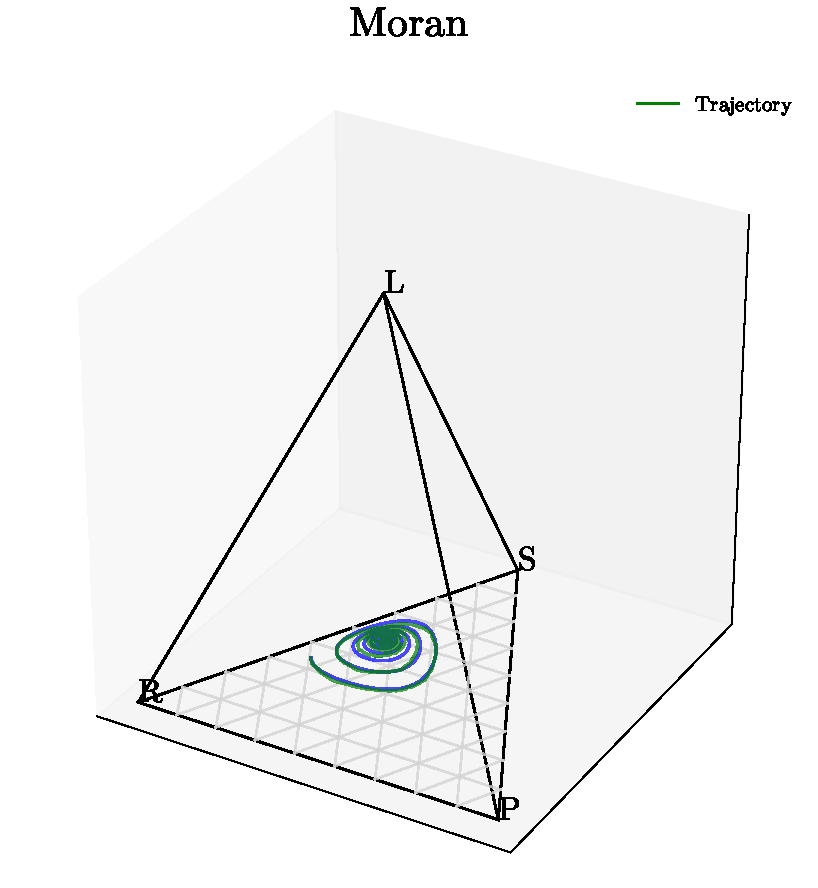
\includegraphics[scale=0.6]{Figures/spiral_in_4d.pdf}
\caption{\label{fig:arps_spiral_in} Same conditions as 
Fig.~\ref{fig:arps_standard_simplex} however with $c=-0.8$ so the 
trajectories are attracted to the RPS center. Corresponds to 
eigenvalues with both real negative part (attracting) and 
complex part spiralling towards the sink. Both the 
numerical solution to the deterministic replicator equations, and a high population
simulated trajectory (green). Strong match between the two.}
\end{figure}

\begin{figure*}
\centering
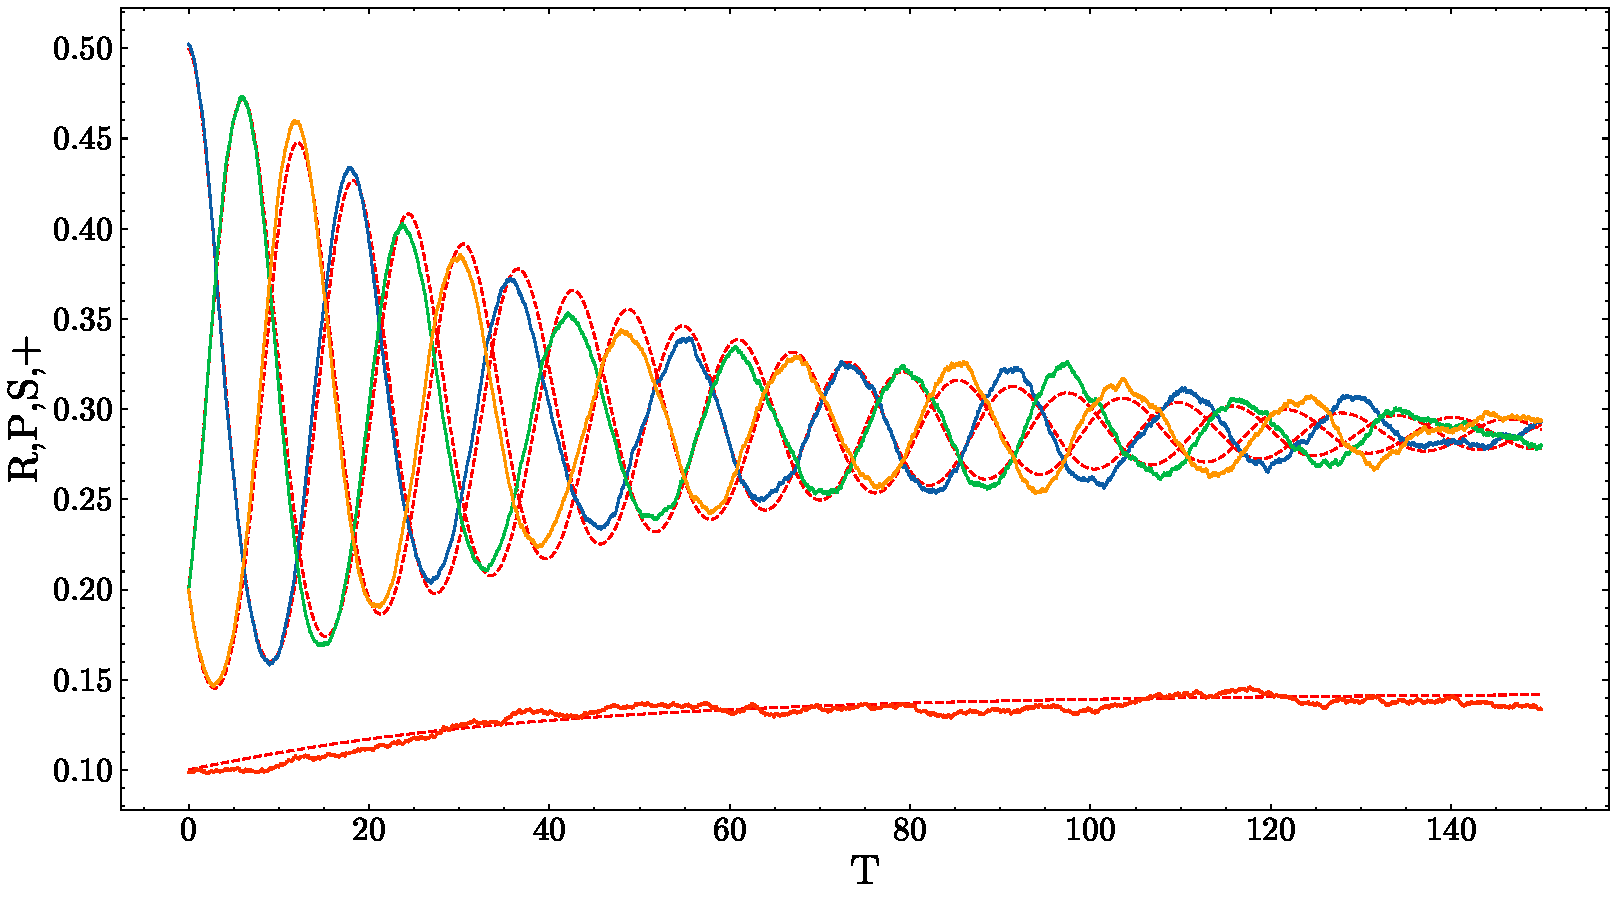
\includegraphics[scale=0.6]{Figures/spiral_in_time_series.pdf}
\caption{\label{fig:arps_spiral_in_time_series} Time series, for the same data plotted in 
Fig.~\ref{fig:arps_spiral_in}, dashed line corresponds to the solved system of ODE's from the 
Moran adjusted dynamics, $a(x)$ from the Fokker-planck derivation.
Amplitude of RPS time series trajectory decays over time as the RPS game 
approaches the interior fixed point.}
\end{figure*}



\section{Model and Stochastic Dynamics}
We consider a finite population of size $N$ evolving under stochastic evolutionary dynamics with $S$ strategies.
The population state is described by the vector 
$\mathbf{x} = (x_1,\dots,x_{S-1})$, where $x_i = n_i/N$ 
and the final strategy is fixed by normalization.
At each update step, individuals interact according to a 
payoff matrix $\mathbf{A}$ and reproduce according to a 
specified microscopic update rule.

Three microscopic update processes are considered: the Moran process,
the local update process, and the local fermi process. Each is defined with a 
reproductive function $\phi$ introduced in the following section and implemented in the 
file.~\cite{aug_rps} ($aug\_rps.py$) responsible for the numerical deterministic 
solutions for the three processes.

In the large--$N$ limit, the stochastic dynamics can be
 approximated by a Fokker--Planck equation governing the 
 probability density $P(\mathbf{x},t)$. 
I will focus on three different stochastic processes to 
model the interactions between the agents, the Moran process,
the local update process and the local fermi process.
Regardless of process, at each time step one individual will 
be selected and reproduce according the different schemes definition
so that the population size remains constant over time.
Mutation can also be considered where individuals have a 
small chance of randomly hopping to another strategy, preventing 
total extinction and the corresponding dynamics 
can be derived for example in Ref.~\cite{general_moran_process} 
a general Moran process
including mutation has been derived.
For simplicity I have not included mutation in the models 
and the effects of finite populations and the phenomenon of 
drift reversal are still clear. Due to the 
ensemble averaging of trajectories often the extinction cases
disappear when multiple simulated runs are combined.



\section{\label{sec:interaction_processes}Interaction processes}

To study the dynamics in finite populations, an interaction process is required for 
comparison between selected agents at each time step.

A generalized form of the Moran process in terms of transition probabilites between states in the 
game simplex has been discussed in Ref.\cite{general_moran_process} and I have implemented in the
simulation code for this project for any number of strategies. Later these transition probabilities can be used to derive a master equation \cite{alma9933506044604871} which 
can be expanded using a Taylor series approximation of the transition probabilities to derive an equation in the form of a Fokker-Planck equation
describing the time evolution of the probability densities of the population states.

The Moran process models evolution as a birth death process where at each update step
one individual is chosen proportional to their fitness in the population for 
reproduction, and one individual is chosen to be killed and replaced by the
strategy of the chosen individual. For the selection process individuals need to have
access to a global average population fitness as individuals are chosen 
relative to their fitness in the whole population. 

In the context of the combined game the probability of switching from one strategy
to another in the Moran process (specifically $R \rightarrow +$) is defined as:

\begin{equation}
    T^{R \rightarrow +} = \frac{1}{2} \frac{1 - w + w \pi_+}{1 - w + w \langle \pi \rangle} \frac{i}{N} \frac{N - i - j - k}{N}
\end{equation}

where $R,+$ denote rock and the 4th strategy and there is $i$ rock players, 
and $N-i-j-k$ $(+)$ players.

And transitions within the RPS game will are of the form:

\begin{equation}
    T^{R \rightarrow S} = \frac{1}{2} \frac{1 - w + w \pi_S}{1 - w + w \langle \pi \rangle} \frac{i}{N} \frac{k}{N}
\end{equation}  
where $w$ is the strength of selection, how much the fitness of an individual 
plays a role in reproduction vs random selection. In weak selection 
limit where $w \rightarrow 0$, this transition probability just becomes 
$\frac{1}{2}\frac{N_i N_j}{N^2}$, and selection is purely random.

The transitions between the other strategies are just permutations of the above
with the corresponding payoffs and populations. $T^{R \rightarrow +}$ will be 
simply written as $T^{R+}$, and similarly for other transitions from here.


Another model is the local update process which considers two 
randomly selected individuals $a,b$ in the population, and individual
$b$ transitions to individual $a$'s strategy with a probability proportional to 
their difference in payoff. Unlike the Moran process this does not require
every individual to know the global average payoff as reproduction 
is decided purely based on local interactions.


Individual $b$ switches to $a$'s strategy with probability:
\begin{equation}
p = \frac{1}{2} + \frac{w}{2} \frac{\pi_a - \pi_b}{\Delta \pi_{max}}
\end{equation}

The transition probability of switching strategy is then:

\begin{equation}
  T^{R \rightarrow +} = \left (\frac{1}{2} + \frac{w}{2} \frac{\pi_+ - \pi_R}{\Delta \pi_{\text{max}}} \right ) \frac{i}{N} \frac{N - i - j - k}{N}
\end{equation}

Where $\Delta \pi_{max}$ is the maximum difference in payoff for the payoff matrix.
In the standard RPS case where $\gamma, \beta < 1$, this is two as the maximum difference
is the difference between an RPS win and loss.


The final model considered is a local
fermi process, similar to the local update process where only 
payoffs between two individuals are compared.

Probability of individual $b$ taking $a$'s strategy is:

\begin{equation}
p = \frac{1}{1 + e^{-w(\pi_a- \pi_b)}} \nonumber
\end{equation}

And 


\begin{equation}
T^{R \rightarrow +} = \left( \frac{1}{1 + e^{-w(\pi_a - \pi_b)}}\right) \frac{i}{N} \frac{N-i-j-k}{N}
\end{equation}


\subsection{General form}

A general form for the transition probability between any two 
strategies can be given by:

\begin{equation}
  \phi(b \rightarrow a) \frac{N_a N_b}{N^2} \nonumber
\end{equation}

Where a reproductive function $\phi$ is defined for each process.
This is how it is implemented in augrps file, with functions
to create a transition probabilities dictionary given a suitable reproduction 
function that meets the interface \cite{aug_rps}. 


\begin{align}
\phi_{MO}(\pi_a, \langle \pi \rangle, w) &= \frac{1}{2} \frac{1 - w + w \pi_a}{1 - w + w \langle \pi \rangle} \\
\phi_{LU}(\pi_a, \pi_b, w) &= \frac{1}{2} +  \frac{w}{2} \frac{\pi_a - \pi_b}{\Delta \pi_{max}} \\
\phi_{FP}(\pi_a, \pi_b, w) &= \frac{1}{1 + e^{-w(\pi_a - \pi_b)}}
\end{align}


\section{\label{sec:fokker-planck} Fokker-Planck Equation}

The Master equation \cite{alma9933506044604871} often used to 
describe particle motion can be derived for this 
system using the transition probabilities of hopping between the 
discrete states.
Using the 2nd order taylor expansion of the transition probabilities
for each strategy, a Fokker-Planck equation can be derived for each of the processes.


The master equation defines the time evolution of a probability density function
for being in any particular state, 
and using the Kramers-Moyal expansion a Fokker-Planck equation can be formed, 
consisting of a drift term and a noise term, and in this case
determinitic replicator dynamics, and stochastic noise from finite $N$.

The master equation \cite{alma9933506044604871} for rock (R) is defined as:

\begin{align}
P^{\tau + 1}(i) - P^\tau(i) &= P^\tau(i-1)T^{PR}(i-1) \nonumber\\
& - P^\tau(i)T^{PR}(i) + P^\tau(i-1)T^{SR}(i-1) \nonumber\\
& - P^\tau(i)T^{SR}(i) + P^\tau(i-1)T^{+R}(i-1) \nonumber\\
& - P^\tau(i)T^{+R}(i) + P^\tau(i+1)T^{RP}(i+1) \nonumber\\
&- P^\tau(i)T^{RP}(i) + P^\tau(i+1)T^{RS} \nonumber \\
&- P^\tau(i)T^{RS}(i) + P^\tau(i+1)T^{R+} \nonumber\\
&- P^\tau(i)T^{R+}(i)
\end{align}
Where $i$ is the number of rock players.
This is composed of transition probabilites into and out of the 
strategy R and describes the time evolution of the system 
jumping between discrete states (the count of $i$ rock individuals).



Expanding the probabilities and the transition probabilites to the 
second order using a Taylor expansion, a Fokker-Planck equation 
can be obtained.

For full derivation of the Fokker-Planck equation for this system,
see the appendix.


Expanding about the rock population fraction $x \pm 1/N$, 
plus or minus 1 individual ($1/N$):
\begin{equation}
  T(x\pm\frac{1}{N}) = T(x) \pm \frac{1}{N}T'(x) + \frac{1}{2N^2}T''(x)\dots \nonumber
\end{equation}
\begin{equation}
  P(x\pm\frac{1}{N}) = P(x) \pm \frac{1}{N}P'(x) + \frac{1}{2N^2}P''(x)\dots \nonumber
\end{equation}
Higher order terms are ignored.

The 2nd order expansions are then subtituted into the Master equation
for the corresponding $\pm$ individual states leading to the 
simplified equation:

\begin{align}
&P^{\tau+1}(x)-P^\tau(x) = \frac{1}{N}\Big[
    -\big(P^\tau(x)\big(
          T^{PR} + T^{SR} + T^{+R} \nonumber \\
        &- T^{RP} - T^{RS} - T^{R+}
      \big)\big)'
\nonumber \\[6pt]
 &+ \frac{1}{2}\big(
      P^\tau(x)\big(\frac{T^{PR}+T^{SR}+T^{+R}
       + T^{RP} +T^{RS}+T^{R+}}{N}\big)
    \big)'' \Big]
\end{align}


This is a Fokker-planck equation of the form:

\begin{equation}
\frac{d}{dt}P^\tau(x)
=
\frac{1}{N}
\left[
-\frac{d}{dx}\!\left(a(x)P^\tau(x)\right)
+ \frac{1}{2}\frac{d^2}{dx^2}\!\left(b^2(x)P^\tau(x)\right)
\right]
\end{equation}
Here $x$ is the fraction of rock players in the population, however, 
the formula is the same for scissors and paper with 
their corresponding $a(y), b(y)$ for paper,
$a(z), b(z)$ for scissors and $a(q), b(q)$ for $+$.

For rock:
\begin{equation} \nonumber
\begin{aligned}
a(x) &= T^{PR} + T^{SR} + T^{+R}
       - T^{RP} - T^{RS} - T^{R+} \\
b(x) &= \sqrt{\frac{1}{N}
\left(
T^{PR} + T^{SR} + T^{+R}
+ T^{RP} + T^{RS} + T^{R+}
\right)}
\end{aligned}
\end{equation}

The term
$a$ is a difference of ingoing and outgoing 
transition probabilities into the particular state and 
$b$ is a noise term consisting of the summation of 
all ingoing plus outgoing transition probabilities. 

Values of $a,b$ for each strategy not included as they are just 
permutations of the above with the respective ingoing/outgoing
transition probabilites for the different strategies. To see 
these in full and the full derivation of the Fokker-Planck
equation refer to the appendix.


For each strategy, $a(x)$ corresponds to the deterministic replicator equation ($N \rightarrow \infty$),
and $b(x)$ is the diffusion term corresponding to the stochastic drift. 
For the local update process, this $a(x)$ is equal to the standard replicator payoff difference equation~\cite{evolution_pop_dynamics}
(with some scaling factor accounting for selection pressure $w$),
whereas the Moran process corresponds to the adjusted dynamics proposed by John Maynard 
Smith~\cite{evolution_maynard}, 
where there is an additional normalization by the average payoff of the population.
Maynard discussed whether the standard dynamics were too restrictive for cases
where fitness is frequency dependent (in a finite population), and therefore proposed the 
adjusted dynamics where you can imagine an individual playing against the population as a whole
via the average payoff term.

A langevin equation describing the trajectory of a single individual in the
game, essentially a stochastic replicator equation follows from this:

\begin{equation}
\dot{x} = a(x) + b(x) \xi
\end{equation}

When plotting a time series of a particular interaction process simulation,
the deterministic dynamics (infinite N) comparison can be made by 
ignoring the noise term $b(x)$ as it contains a factor $1/N$, and 
solving numerically $a(x)$ which corresponds to the deterministic 
replicator dynamics for that interaction process.

\subsection{Deterministic dynamics}

Considering $a(x)$ for the different processes shows
that for the Moran process, it corresponds to the adjusted 
replicator dynamics considered in Ref.\cite{evolution_maynard} as shown in 
Ref.\cite{drift_reversal_paper}.

\begin{equation}
\dot{x}_{MO} = \frac{1}{\Gamma + \langle \pi(x)\rangle} x_i(\pi_i(x) - \langle \pi(x)\rangle)
\end{equation}
where $\Gamma = \frac{1- w}{w}$, see full expanded form in the appendix~\cite{project_appendix}.

The local update process corresponds to the standard replicator 
dynamics \cite{evolution_pop_dynamics} used in section
\ref{RPS-model} and \ref{SD-model} to define the deterministic dynamics
for RPS and SD but with an additional scaling by the
constant selection pressure
$w$ which was not considerd in infinite $N$ scenarios.
The scaled dynamics for the local update process results in the following equation:

\begin{equation}
\dot{x}_{LU} = \frac{w}{\Delta \pi_{max}}x_i(\pi_i(x) - \langle \pi(x) \rangle)
\end{equation}
which is the $a(x)$ part of the local update process Fokker-Planck equation.


The fermi process adjusted replicator equation in the deterministic limit 
of $N \rightarrow \infty$ is defined as the pairwise difference form of the 
replicator dynamics:
\begin{align}
\dot{x}_{FE} &= x \Big[
    y \tanh\!\left(\frac{w(\pi_R - \pi_P)}{2}\right)
  + z \tanh\!\left(\frac{w(\pi_R - \pi_S)}{2}\right)\nonumber \\
  &+ q \tanh\!\left(\frac{w(\pi_R - \pi_+)}{2}\right)
\Big]
\end{align}

Each of these are verified against the Fokker-Planck term $a(x)$ using the symbolic mathematics library sympy available in 
File.~\cite{aug_rps}. These equations describe the deterministic limit of $N \rightarrow \infty$ of the replicator
dynamics
for each microscopic interaction processes.
The following sections will explore the effects of the stochastic diffusion term $b(x)$ by defining a set of 
drift observables, and exporing low $N$ cases.



\section{\label{sec:drift_measures}Drift Measures}

A measure of the drift from the internal fixed point of this system can be defined by
an observation function $H$ \cite{Claussen2007-zo,drift_reversal_paper,rps_cyclic_jens}, and 
approximating the value of $\dot{H}$ with a discrete sum over the population.
Previous work in Ref. \cite{Claussen2007-zo,drift_reversal_paper,rps_cyclic_jens} has
examined this both the 2 and 3 strategy case where only one observable $H$ is used, however
to analyze the combined game an observable will be defined for each of the sub games to 
properly describe the dynamics and drift. These will be $H_{SD}, H_{RPS}$, and $H_4$ 
as approximation of the distance from the SD equilibrium , the RPS equilibrium and then the 
overall central equilibrium as a whole respectively.

An approximation for $\dot{H}$, $\langle \Delta H \rangle$ can be computed directly from the 
agent based simulation, however for all the interaction processes the terms can be 
formulated as an integral and solved numerically on in some cases e.g. Local update, a 
closed form solution can be found. This is preferred over simulated approximate values as it is much 
simpler to compute particularly in the local update case where an exact result can be found 
for $\langle \Delta H \rangle$. 
For each of the components making up the combined $4 \times 4$ game a suitable observation
value $H$ can be defined to measure the distance from the Nash equilibrium 
\cite{drift_reversal_paper,rps_cyclic_jens}. The sign of $\dot{H}$ can therefore
indicate whether the system is drifts towards or away from the interior equilibrium \cite{drift_reversal_paper}.
$\dot{H}$ is approximated in the simulated results by $\langle \Delta H \rangle$:

\begin{equation}
\langle \Delta H \rangle = \mathbb{E}[H(\mathbf{x}_{t+1}) - H(\mathbf{x}_t)].
\end{equation}

which is calculated for one single update step, and then averaged over a very large number of 
repeated simulations. Drift reversal is defined as the change in sign of this value under
variation of parameters of the system most notably the population size N. 

The sign of $\langle \Delta H \rangle$ determines whether stochastic drift favors interior coexistence or boundary attraction.
$\langle \Delta H \rangle$ can be formulated analytically \cite{rps_cyclic_jens} and
written as a sum over the simplex, in this case:
($1 \le i, j \le N -i, k \le N - i - j$).

\begin{equation}
\langle \Delta H \rangle = \sum_{i=1}^{N} \sum_{j=1}^{N-i} 
\sum_{k=1}^{N-i-j} \left(H_{s} - H_{s^\prime}\right)T^{s
\rightarrow s^\prime}
\end{equation}
for all the states $s, s^\prime \in \{R, P, S, L\}$ and transition probabilities $T^{s \rightarrow s^\prime}$.
Where transition probabilites $T^{s \rightarrow s'}$ must be defined for each of the 
microscopic interaction processes. In the combined SD, RPS game there are 3 observation values
for drift, $H_{SD}$ for effects within the snowdrift game, $H_{RPS}$ for the RPS subgame and 
$H_4$ for the overall drift in the context of the internal fixed point of all 4 strategies in the 
payoff matrix. 

After defining the summation in terms of discrete population counts for each of the 
strategies, it is possible to approximate these values in the continuous limit by replacing
the counts with their corresponding fraction of the population and the term is converted to 
an integral over the simplex allowing for the use of numerical methods to compute these
exact values of $\langle \Delta H \rangle$, and therefore compute numerically the 
critical population sizes $N$ where the dynamics shift and drift reversal occurs (if it does occur).
This allows for more efficient comparisons of the dynamics of a particular instance of the game parameters
as it is much more efficient to compute this equation numerically than to simulate over a large number of
realizations and average the discrete results.


\subsection{Snowdrift Drift}

The 4th strategy occurs with frequency $q = 1 - x - y - z$, 
we define the snowdrift coexistence measure

\begin{equation} \label{eq:H_SD}
H_{SD} = - q(1-q)
\end{equation}

The expected value of $\Delta H_{SD}$ over the entire simplex 
can be defined, similarly to the RPS case, by 
a sum as follows:


\begin{widetext}
\begin{equation}
\begin{aligned}
\langle \Delta H_{\mathrm{SD}} \rangle 
&= \frac{6}{N^5} \sum_{i=1}^{N} \sum_{j=1}^{N-i}  \sum_{k=1}^{N-i-j}  \Big[(N-i-j-k)(1-N+i+j+k)(T^{R+} + T^{P+} + T^{S+}+ T^{+R}+ T^{+P} +T^{+S}) \\
&- (N-i-j-k + 1)(-N+i+j+k)T^{R+} - (N-i-j-k + 1)(-N + i + j + k)T^{P+} \\
&- (N-i-j-k - 1)(2 - N + i + j + k)T^{+R} - (N - i - j - k - 1)(2 - N + i + j + k)T^{+P} \\
&- (N - i - j - k - 1)(2 - N + i + j + k)T^{+S}\Big]
\end{aligned}
\end{equation}
\end{widetext}

the sum can be converted into the following continuous form where
$x = i/N, y= j/N, z=k/N$. See derivation for this transition in full 
in the appendix.

\begin{align}\label{eq:delta_h_sd}
\langle \Delta H_{\mathrm{SD}} \rangle 
&= \frac{12}{N} \int_{0}^{1} dx \int_{0}^{1-x}dy 
\int_{0}^{1-x-y}dz \\ \nonumber
\Big[& q \big[ 
(T^{R+} - T^{+R}) + (T^{P+} - T^{+P}) \\\nonumber
+& (T^{S+} - T^{+S}) \big] \Big] \\\nonumber
+& \frac{12}{N^2} \int_{0}^{1} dx \int_{0}^{1-x}dy 
\int_{0}^{1-x-y} dz \\ \nonumber
\Big[& T^{+R} + T^{+P} + T^{+S} \Big] 
\end{align}


Since transitions purely within the RPS subgame do not change the value
of $H_{SD}$, this exact term for depends only on transitions into and out of 
the fourth strategy ($+$). 

Consider the case of 
$(H_{SD} - H_{SD}')T^{RP}$ in the summation being zero, since transitions between 
rock and paper do not change the frequency of the fourth strategy, and therefore
do not change the value of $-q(1-q)$. 

This results in $H_{SD} - H_{SD}' = H_{SD} - H_{SD} = 0$ for all transitions
($R \rightarrow P, P \rightarrow S, S \rightarrow R$,
and their reverses) within the RPS subgame. For full
derivation see the appendix\cite{project_appendix}.



\subsection{Rock-Paper-Scissors Drift}
For the three-strategy subsystem, the replicator equations have the constant of motion:
\begin{align}
H_{\mathrm{RPS}} = - x y z
\end{align}
which is a measure of the distance of a populaton from the internal fixed point of RPS.



$\langle \Delta H_{RPS} \rangle$ is approximated by a sum:

\begin{align}
  \langle \Delta H_{RPS} \rangle &=
  \frac{2}{N^6} \sum_{i=1}^{N}\sum_{j=1}^{N-i}\sum_{k=1}^{N-i-j}\Big[
  ijk(T^{RP} + T^{RS} + T^{R+} \nonumber \\
  & + T^{PR} + T^{PS} + T^{P+} + T^{SR} + T^{SP} + T^{S+} \nonumber \\
  & + T^{+R} + T^{+P} + T^{+S}) - k(i-1)(j+1)T^{RP} \nonumber \\
  &- (i-1)j(k+1)T^{RS} - jk(i-1)T^{R+} \nonumber\\
  &- k(i+1)(j-1)T^{PR} - i(j-1)(k+1)T^{PS} \nonumber \\
  & - ik(j-1)T^{P+} - (i+1)j(k-1)T^{SR} \nonumber \\
  & - i(j+1)(k-1)T^{SP} - ij(k-1)T^{S+} \nonumber \\
  &- jk(i+1)T^{+R} - ik(j+1)T^{+P} \nonumber \\
  &- ij(k+1)T^{+S}\Big]
\end{align}
the sum can be converted into the following continuous form where
$x = i/N, y= j/N, z=k/N$. See derivation for this transition in full 
in the appendix.


\begin{align}
\langle \Delta H_{\mathrm{RPS}} \rangle
&= \frac{2}{N} \int_{0}^{1}dx 
\int_{0}^{1-x}dy
\int_{0}^{1-x-y}dz \nonumber\\
\Big[ 
&z (y-x) (T^{RP} - T^{PR}) \nonumber\\
+& y (z-x) (T^{RS} - T^{SR}) \nonumber\\
+& x (y-z) (T^{SP} - T^{PS}) \nonumber\\
+& xz(T^{P+} - T^{+P}) + yz(T^{R+} - T^{+R}) \nonumber\\
+& xy(T^{S+} - T^{+S})
\Big] \nonumber\\
+& \frac{2}{N^2} \int_{0}^{1}dx \int_{0}^{1-x}dy
\int_{0}^{1-x-y}dz \nonumber\\
\Big[
&z(T^{RP} + T^{PR}) + y(T^{RS} + T^{SR}) \nonumber\\
+& x(T^{SP} + T^{PS})
\Big]
\end{align}

The RPS drift is therefore controlled by differences of 
transition probabilites between the RPS states as in 
\cite{rps_cyclic_jens} with additional terms in and out of the 
RPS game itself to the 4th strategy.




\subsection{Four-Strategy Coexistence Drift}

\par
To capture full four-strategy coexistence, the constant of motion $H_4$ is defined
\begin{equation}
H_4 = - x y z q 
\end{equation}
which vanishes on all faces of the simplex and is maximized in the interior.


The expected value of $\Delta H_4$ can be defined as the sum over all the states below
\begin{widetext}
\begin{equation}
\begin{aligned}\label{eq:delta_h_4}
\langle \Delta H_{4} \rangle &= \frac{6}{N^7} \sum_{i=1}^{N} \sum_{j=1}^{N-i}  \sum_{k=1}^{N-i-j} \Big[ijk(N-i-j-k)
(T^{RP} + T^{RS} + T^{R+} + T^{PR} + T^{PS} + T^{P+} \\
&+ T^{SR} + T^{SP} + T^{S+} + T^{+R} + T^{+P} + T^{+S}) - (i-1)(j+1)k(N-i-j-k)T^{RP} \\
&- (i-1)j(k+1)(N-i-j-k)T^{RS} - (i-1)jk(N-i-j-k + 1)T^{R+} \\
&- (i+1)(j-1)k(N-i-j-k)T^{PR} - i(j-1)(k+1)(N-i-j-k)T^{PS} \\
&- i(j-1)k(N-i-j-k + 1)T^{P+} - (i+1)j(k-1)(N-i-j-k)T^{SR} \\
&- i(j+1)(k-1)(N-i-j-k)T^{SP} - ij(k-1)(N-i-j-k + 1)T^{S+} \\
&- (i+1)jk(N - 1 -i-j-k)T^{+R} - i(j+1)k(N - 1-i-j-k)T^{+P} - ij(k+1)(N - 1-i-j-k)T^{+S}\Big]
\end{aligned}
\end{equation}
\text{In the continuous limit}
\begin{equation}
\begin{aligned}
\langle \Delta H_{4} \rangle &= \frac{6}{N} \int_{0}^{1}dx \int_{0}^{1-x} dy \int_{0}^{1-x-y}dz 
\Big[zq(y - x)(T^{RP} - T^{PR}) + yq(z - x)(T^{RS} - T^{SR}) +xq(y-z)(T^{SP} - T^{PS}) \\ 
&+ yz(q-x)(T^{R+} - T^{+R}) + xz(q-y)(T^{P+} - T^{+P}) + xy(q-z)(T^{S+} - T^{+S})\Big] \\
&+ \frac{6}{N^2} \int_{0}^{1}dx \int_{0}^{1-x} dy \int_{0}^{1-x-y}dz\Big[zq(T^{RP} + T^{PR}) + yq(T^{RS} + T^{SR}) + xq(T^{SP} + T^{PS}) \\
&+ yz(T^{R+} + T^{+R}) + xz(T^{P+} + T^{+P}) + xy(T^{S+} + T^{+S})\Big]
\end{aligned}
\end{equation}
\end{widetext}
This expression naturally decomposes into RPS--like drift terms, snowdrift--like drift terms, and diffusion corrections.
The sign of $\langle \Delta H_4 \rangle$ determines whether stochastic dynamics favors four--strategy coexistence or boundary attraction.


\subsection{Weak selection limit}

Considering the weak selection limit where $w \rightarrow 0$, terms of the form 
$T^{R+} - T^{+R}$ vanish, so for the SD drift measure only the terms under $1/N^2$ are left.

The sum $T^{+R} + T^{+P} + T^{+S}$ simplifies to:

\begin{align}
T^{+R} + T^{+P} + T^{+S} &= \frac{1}{2}\frac{N-i-j-k}{N}\left(\frac{i}{N} + \frac{j}{N} + \frac{k}{N}\right) \nonumber \\
= \frac{1}{2}q(x+y+z) &= \frac{1}{2}(1-x-y-z)(x+y+z) \nonumber 
\end{align}

Therefore $\langle \Delta H_{\mathrm{SD}} \rangle$ becomes (when $w \rightarrow 0$):

\begin{align}\label{eq:delta_h_sd_weak}
\langle \Delta H_{\mathrm{SD}} \rangle_{w \rightarrow 0} 
&= \frac{12}{N^2} \int_{0}^{1} dx \int_{0}^{1-x}dy 
\int_{0}^{1-x-y} dz \nonumber \\ 
\Big[&  \frac{1}{2}(1-x-y-z)(x+y+z) \Big] \nonumber \\
&= \frac{3}{20N^2}
\end{align}


As $w \rightarrow 0$ the three values of $\langle \Delta H_{SD} \rangle$ as
population size varies will approach this limit as seen in 
Fig.~\ref{fig:weak_selection_comparison} and a drift reversal will no longer occur as the critical population size is undefined since
$\frac{3}{20N^2} \ne 0$ at any point since $N \in \mathbb{N}$. However in the linear in $w$ case even for weak selection 
where $w << 1/2$ a drift reversal is possible for each of the processes.


\begin{figure}[t]
\centering
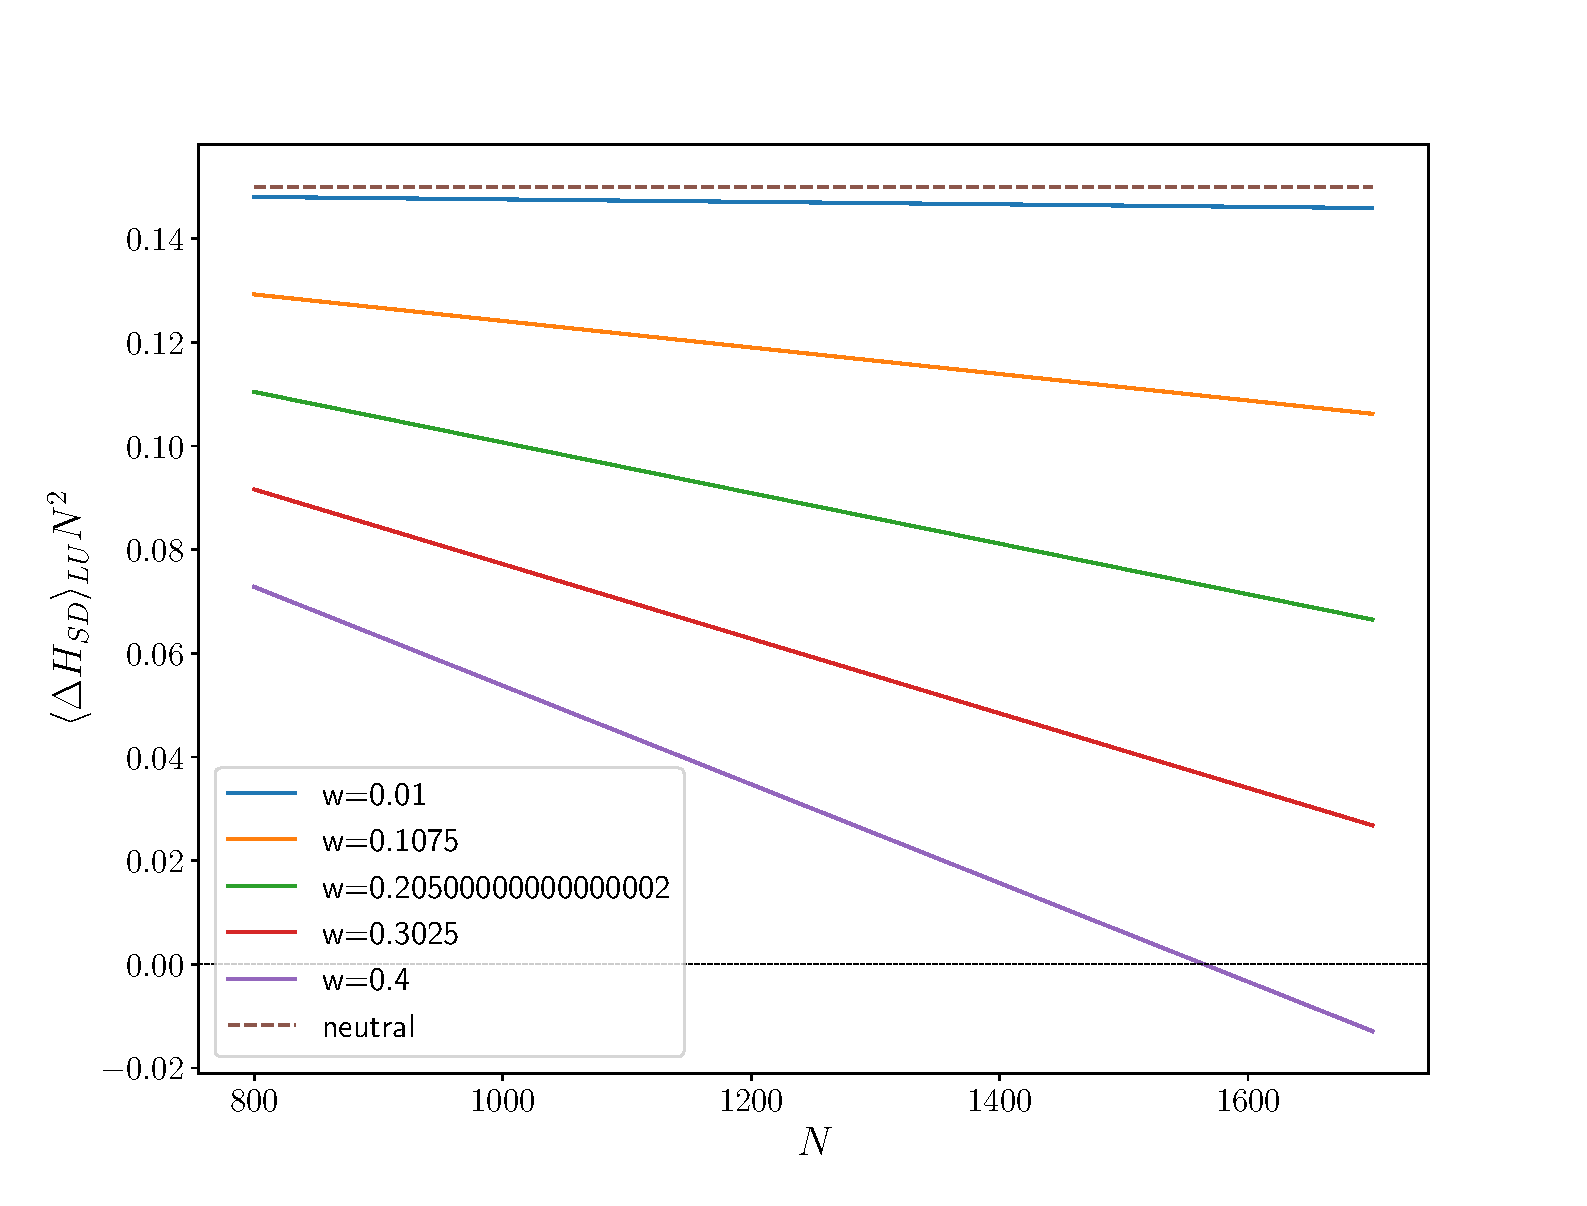
\includegraphics[width=0.45\textwidth]{Figures/weak_selection_comparison.pdf}
\caption{\label{fig:weak_selection_comparison} Plot of $\langle \Delta H_{\mathrm{SD}} \rangle_{LU}$ for 
varying $N$ and different values of $w$ approaching the limit $w \rightarrow 0$.
A drift reversal occurs for 
all $w > 0$ under the initial parameters, $a = 0, b = 1, c=-0.2, \gamma = 0.14, \beta = 0.3$, 
as values approach and eventually intersect with dashed line $\langle \Delta H_{\mathrm{SD}} \rangle_{LU} = 0$.}
\end{figure}
For $\langle \Delta H_{RPS} \rangle$, the terms of the form $T^{RP} - T^{PR}$ vanish, and the 
integral scaled by $2/N^2$ reduces to:

\begin{align} \label{eq:weak_selection_rps}
\frac{2}{N^2} \int_{0}^{1}dx\int_{0}^{1-x}dy\int_{0}^{1-x-y}dz\left(3xyz\right) \nonumber\\
= \frac{1}{120N^2}
\end{align}
like the SD observable, in the weak selection limit there is also no drift reversal as $\langle \Delta H_{RPS} \rangle$
does not change sign, however for $w > 0$, it is possible depending on the parameters of the system.


In the weak selection limit the difference in payoff between the strategies has little effect on 
reproduction relative to the random drift. This corresponds to the theory of neutral evolution which is popular in 
molecular evolution and states that the majority of evolution at the molecular level is governed by random drift as opposed
to the differences in payoffs, or fitness of the individuals in the population.

\subsection{\label{section:local_analytical}Local update analytical solutions}


For the Local update process, an exact solution for the values 
$\langle \Delta H_{SD} \rangle$ and $\langle \Delta H_{RPS} \rangle$
can be found.

Considering the payoff matrix:
\begin{align} \label{SimplifiedRPS}
\begin{bmatrix}
    0 & c & 1 & \gamma\\
    1 & 0 & c & \gamma\\
    c & 1 & 0 & \gamma\\
    \beta & \beta & \beta & 0
\end{bmatrix}
\end{align}
In this case the values of $a,b$ have been set to 0 and 1. The value of $c$ can be
altered to adjust the dynamics of the RPS component of the game, if $c > -1$
then the game will spiral inwards towards a central fixed point and if $c > - 1$
the RPS trajectories will sprial outwards as shown in the introductory section.
The values of $\beta$ and $\gamma$ determine the dynamics of the snowdrift component of the 
game with the main cases being fixation at either the top (pure 4th strategy), base (pure RPS) or a central equilibrium.
This depends on the relative payoff difference between the SD and RPS game.


$\langle \Delta H_{SD} \rangle$ is composed of differences of the form 
$T^{R+} - T^{+R}$. Expanding these differences:


\begin{align}
T^{R+} - T^{+R} &= \frac{i}{N}\frac{N-i-j-k}{N}\left(\frac{1}{2} + \frac{w}{2}\frac{\pi_+ - \pi_R}{\Delta \pi_{\text{max}}}\right) \nonumber \\
&- \frac{i}{N}\frac{N-i-j-k}{N}\left(\frac{1}{2} + \frac{w}{2}\frac{\pi_R - \pi_+}{\Delta \pi_{\text{max}}}\right) \nonumber \\
&= w\frac{i}{N}\frac{N-i-j-k}{N}\left(\frac{\pi_+ - \pi_R}{\Delta \pi_{\text{max}}}\right)\nonumber
\end{align}

And then using population frequencies instead of the discrete population counts:


\begin{equation}
T^{R+} - T^{+R} = wx(1-x-y-z)\frac{\pi_+ - \pi_R}{\Delta \pi_{\text{max}}}
\end{equation}

The other transition probability differences are omitted here since they are symmetrical to the above with the 
population count and payoff switched to their respective values.

The second component of $\langle \Delta H_{SD} \rangle$ are the terms in order $1/N^2$, $T^{+R} + T^{+P} + T^{+S}$.

This expression eventually simplfies to the following in terms of $w, \Delta \pi_{max}$ and the payoff
matrix parameters:

\begin{align}
&T^{+R} + T^{+P} + T^{+S} = \nonumber\\ 
&\frac{1}{2}(1-x-y-z)\Bigg[x + y + z + \frac{w}{\Delta \pi_{\text{max}}}  \nonumber\\
&\Big[x(z + cy + \gamma(1 - x - y z) - \beta(x+y+z))  \nonumber\\
&+ y(x + cz + \gamma(1 - x - y z) - \beta(x+y+z))  \nonumber\\
&+ z(y + cx + \gamma(1 - x - y z) - \beta(x+y+z))\Big]
\Bigg] \nonumber
\end{align}

Replacing these in the original integral (equation \ref{eq:delta_h_sd}), the integral can now be solved exactly
leading to:


\begin{align}
\langle \Delta H_{SD} \rangle_{LU} &= \frac{1}{280N^2 \Delta \pi_{max}} \Bigg[42 \Delta \pi_{\text{max}} \nonumber \\
&+ 2w \gamma (7 - 6N) \nonumber\\
&+ (-1+4\beta - c)(-7 + 4N)w \Bigg]
\end{align}



Which is an exact expression for the expected drift for the local update process when observing the SD
component of the game. Since drift reversal is a change in sign in $\langle \Delta H_{SD} \rangle_{LU}$, this 
leads to an exact term for the critical population size by setting this to 0:



\begin{align}
N^\prime_{SD} &= \frac{-42 \Delta \pi_{\text{max}} + w(28\beta - 7c  - 14 \gamma - 7)}{w(16 \beta - 4c -12\gamma - 4)} \nonumber\\
&= \frac{-42 \Delta \pi_{\text{max}}}{w(16 \beta - 4c -12\gamma - 4)}
+ \frac{28 \beta - 7c - 14\gamma - 7}{16 \beta - 4c -12\gamma - 4}
\end{align}






A similar process can be done for the RPS drift observable.

The difference terms $T^{RP} - T^{PR}$ for the local update transition probabilites are of the form:

\begin{align}
T^{RP} - T^{PR} &= \frac{w}{\Delta \pi_{max}}xy(\pi_P - \pi_R)\nonumber \\
&=  \frac{w}{\Delta \pi_{max}}xy(x - z + c(z - y))
\end{align}

The terms factored by $w$ within the expression of the form $T^{RP} + T^{PR}$ cancel out leaving the second integral to be 
the same as in the weak selection limit (equation.~\ref{eq:weak_selection_rps}) giving a constant term 
of $1/120N^2$.



After subtituting in the expanded forms of the transition probability differences, $\langle \Delta H_{RPS} \rangle_{LU}$
eventually simplifies to:

\begin{equation}
\langle \Delta H_{RPS} \rangle_{LU} = \frac{1}{120N^2} 
- \frac{w(2 + \gamma - 3\beta = 2c)}{3360N\Delta \pi_{max}}
\end{equation}
Setting this to 0, an exact solution for the local update critical 
population size is:
\begin{equation}
N^\prime_{RPS} = \frac{28\Delta \pi_{max}}{w(2 + \gamma -3\beta + 2c)}
\end{equation}
Full derivation in appendix~\cite{project_appendix} under analytical solution for Local update process.


\subsection{Drift reversal and comparison of drift measures}



Drift reversal, below a critical
population size, occurs at the point where the 
value of $\langle H \rangle$ changes sign.
Depending on the initial parameters, 
this effect is observed in the RPS and SD subgames, and in some cases
in both in the agent based simulations and also from the 
exact solutions for $\langle \Delta H \rangle$ for the different 
interaction processes and in the case of the local update process, 
exact expressions for the critical population size for a special case 
of the game are derived in section ~\ref{section:local_analytical}.

Fig.~\ref{fig:drift_time_series} demonstrates drift reversal for each of the 
three different update processes on the same game parameters, showing the 
replicator equations solution, the large $N$ case and the low $N$ case where a 
drift reversal occurs and the trajectories on average move in the opposite 
direction predicted by the replicator dynamics.


\begin{figure}[t]
    \centering
    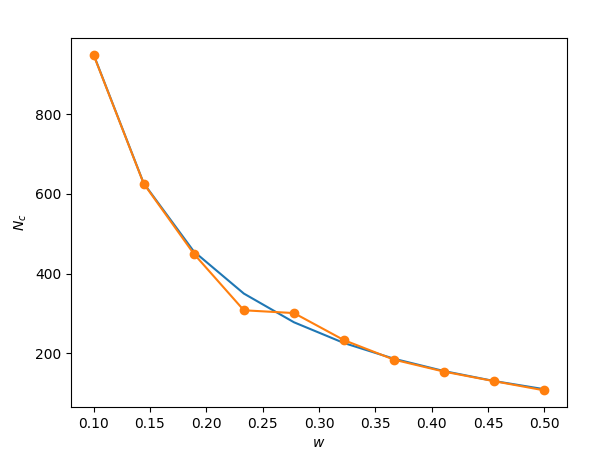
\includegraphics[width=0.4\textwidth]{Figures/critical_n_analytical.png}
    \caption{\label{fig:n_c_against_w}Comparison of simulated critical population sizes against the derived expected change in H for Moran process. Small deviations due
    to stochasticity in the simulations. $\gamma = 0.2, \beta = 0.1$ standard RPS.
    Small deviations due to random nature of simulations, but close match to analytical result.
    Drift reversal is present in the agent based simulations and exactly matching analytical prediction
    for these paremeters. Each point on the simulated values averaged 100,000,000 times.
    Computed through simulations where the drift observable is approximated over one update step and averaged}
\end{figure}


\begin{figure}
    \centering
    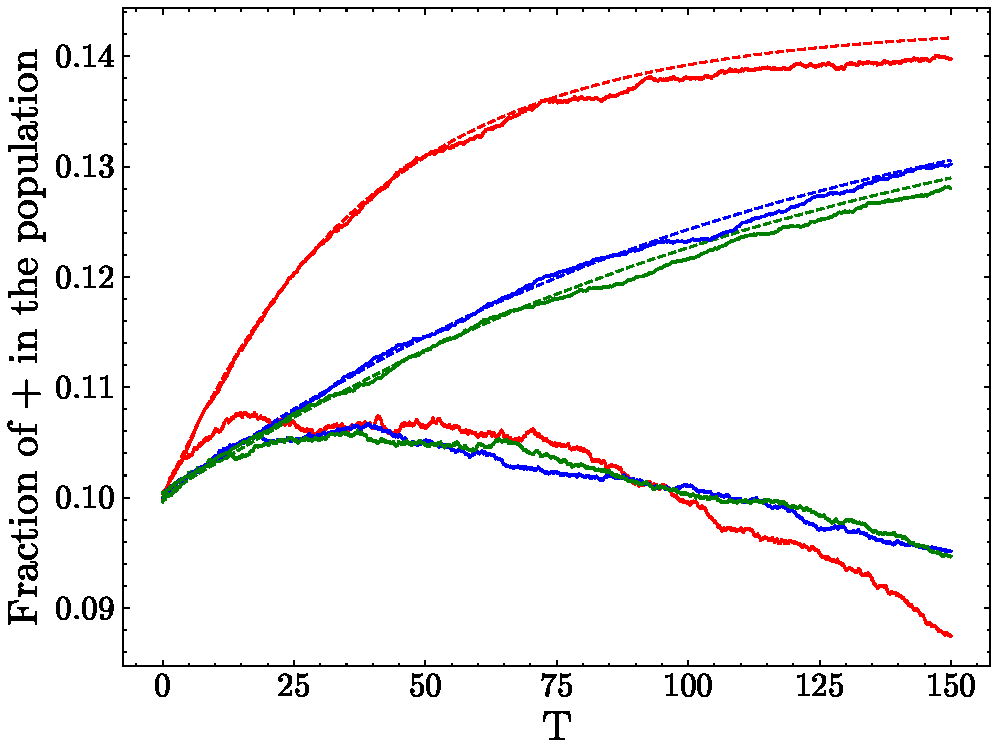
\includegraphics[width=0.4\textwidth]{Figures/proces_drift_time_series.pdf}
    \caption{\label{fig:drift_time_series} A time series comparison for 
    average trajectories of the three processses, 
    Moran (red), local update (blue) and fermi (green). Dashed line is the 
    deterministic solution to their respective adjusted replicator equations.
    Large $N=100000$ simulated results with no drift reversal shown to follow the 
    deterministic trajectory will small deviations due to noise. Low $N=200$ of the 
    same process and parameters averaged over 1000 realizations exhibits drift reversal 
    away from the fixed point predicted by replicator dynamics towards 
    full RPS where the fourth strategy $+$ fraction converges to 0.}
\end{figure}



In either cases this leads to a few notable cases resulting in very 
different dynamics in the multiple game system summarized by
Fig.~\ref{drift_cases_fig}

Assuming a set of parameters where both a critical population size exists
for both the SD and RPS part of the game where $N^\prime_{SD}, N^\prime_{RPS}, N$,
are the critical sizes and the actual population size respectively there
are the cases:


\begin{enumerate}%[itemsep=0mm, parsep=2pt]
  \centering
  \item $N^\prime_{SD} < N < N^\prime_{RPS}$
  \item $N^\prime_{RPS} < N < N^\prime_{SD}$
  \item $N >> N^\prime_{RPS}, N^\prime_{SD}$
  \item $N << N^\prime_{RPS}, N^\prime_{SD}$
\end{enumerate}

In case 1, population size is below the critical size for 
drift reversal in the RPS component, and therefore 
(for an attracting RPS game where $c > -1$) the trajectories would 
gradually move away from the internal fixed point in the RPS plane 
on average where in the large $N$ case they would fixate there.
Since $N$ is larger than the critical size for the SD component there 
would be no reversal in the SD game and the trajectories would follow the 
drift expected from the replicator determinstic dynamics, e.g. the 
center of the vertical column in the 3d 4-simplex projection (for the
setting where there is stable mixed strategy nash equilibrium in SD).
This corresponds to the case in the bottom right of Fig.~\ref{drift_cases_fig}, 
where RPS trajectories fill out the plane and eventually in time are absorbed by 
the RPS boundaries.

In the case where $N^\prime_{RPS} < N < N^\prime_{SD}$ the point cloud of trajectories from 
randomly initialized simulations will be attracted to the equilibrium of the RPS game, but will
exhibit a drift reversal in the SD game, seen in the SD reversal case in Fig.~\ref{drift_cases_fig}.
This case is visible in Fig.~\ref{fig:rps_reversal_case}, where critical population size 
for RPS is much larger than for SD.


Case 2 is the exact opposite of this where a reversal takes place in 
the SD component and not the RPS component resulting in the 
cloud of randomly initialised trajectories to 
fill out a vertical column in the 3d projection as they diverge
from the expected central fixed point for the given payoff matrix (see inset).
Here since $N > N^\prime_{RPS}$ there is no reversal in the RPS component
and since this RPS game is attracting and mutual coexistence is optimal, the 
trajectories remain in the center of the RPS plane meanwhile the SD components
dynamics reverse. See Fig.~\ref{fig:sd_reversal_case} for this case.

The remaining two cases demonstrate the effects of a very large population size 
$N >> N^\prime_{RPS}, N^\prime_{SD}$ where the trajectories
approach that described by the deterministic replicator equations, and 
the trajectories all converge at the internal fixed point. 
And the case where $N$ is very small and there is drift reversal 
in both the subgames so trajectories are moving away from the internal fixed point 
in all directions and are absorbed by the boundaries eventually 
ending in the four corners of the simplex.


\begin{table}[H]
\caption{\label{tab:table1}%
Table of values used for the drift cases graph
Rows marked with * are the cases illustrated in Fig.~\ref{drift_cases_fig}
}
\begin{ruledtabular}
\begin{tabular}{c|c|c|c|c|c}
\textrm{$\alpha$}&
\textrm{$\beta$}&
\textrm{$c$}&
\textrm{$N$}&
\textrm{$N/N_{SD}$}&
\textrm{$N/N_{RPS}$}\\
\colrule
0.1 & 0.1 & -0.8 & 50  & 0.12  & 0.09* \\
0.14 & 0.3 & -0.2 & 200  & 0.14  & 2.26 \\
0.14 & 0.3 & -0.2 & 300  & 0.21  & 3.41* \\
0.4 & 0.2 & -0.8 & 200  & 2.83  & 0.36 \\
0.4 & 0.24 & -0.8 & 600 & 6.28 & 0.42* \\
0.1 & 0.1 & -0.8 & 2000 & 4.76 & 3.57 \\
0.1 & 0.1 & -0.8 & 30000 & 71.43 & 53.57* \\
\end{tabular}
\end{ruledtabular}
\end{table}


The axis $N/N_{RPS}$ and $N/N_{SD}$ are used to 
illustrate the relationship between the 3 population values, 
where both the critical sizes change and also the 
value of $N$ varies since they all impact the dynamics.






\begin{figure}
    \centering
    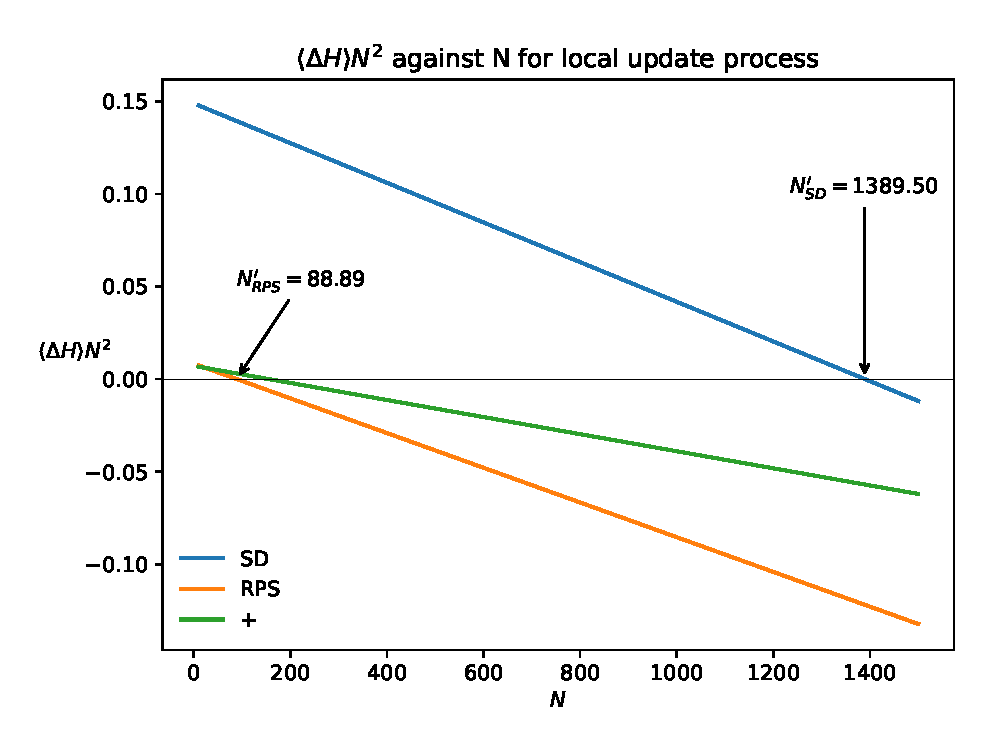
\includegraphics[width=0.4\textwidth]{Figures/column_case_delta_H.eps}
    \caption{\label{fig:sd_reversal_case}
    SD reversal  Comparison of the 3 drift measures $\langle \Delta H_{SD} \rangle,
    \langle \Delta H_{RPS} \rangle, \text{and} \langle \Delta H_+ \rangle$ for the 
    local update process. $\beta = 0.3, \gamma=0.14, c=-0.2$, strong 
    central attracting RPS case ($c > -1$) and $N_{RPS} < N_{SD}$ so 
    SD game component reverses first, at a higher population size.
    This results in the vertical column point cloud where RPS fixates at the 
    central fixed point where $x \approx y \approx z$ and $q$ drifts away from the fixed point ($N_{RPS} < N < N_{SD}$)}
\end{figure}

\begin{figure}
  \centering
  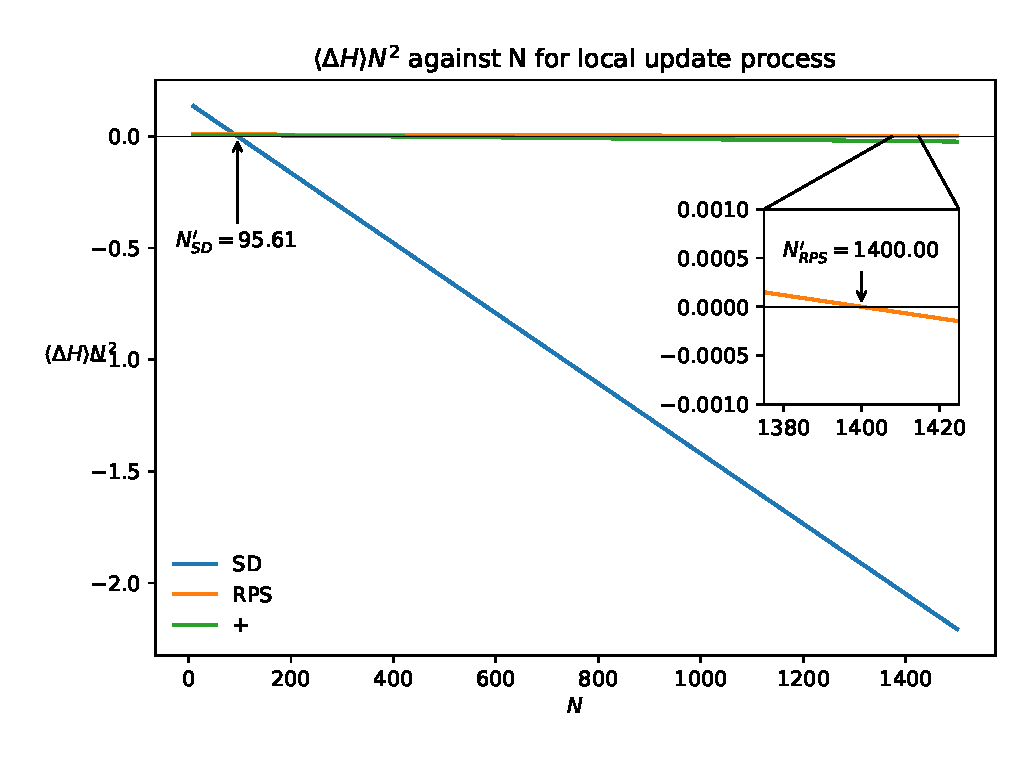
\includegraphics[width=0.4\textwidth]{Figures/disk_clean_deltaH.eps}
  \caption{
    \label{fig:rps_reversal_case}
  RPS reversal $\beta=0.24, \gamma=0.4, c=-0.8$ cleaner disk case, clamped the starting values where $q > 0.1 < 0.9$ to prevent RPS random extinctions for a clearer image.
  This parameter settings give a better  plot becaues $N_{RPS} >> N_{SD}$ for the disk case. $N_{SD} = 95.61, N_{RPS} = 1400$}
\end{figure}




\begin{figure*}[t] 
\centering
\begin{tikzpicture}
  \node[anchor=south west, inner sep=0] (img) at (0,0)
    {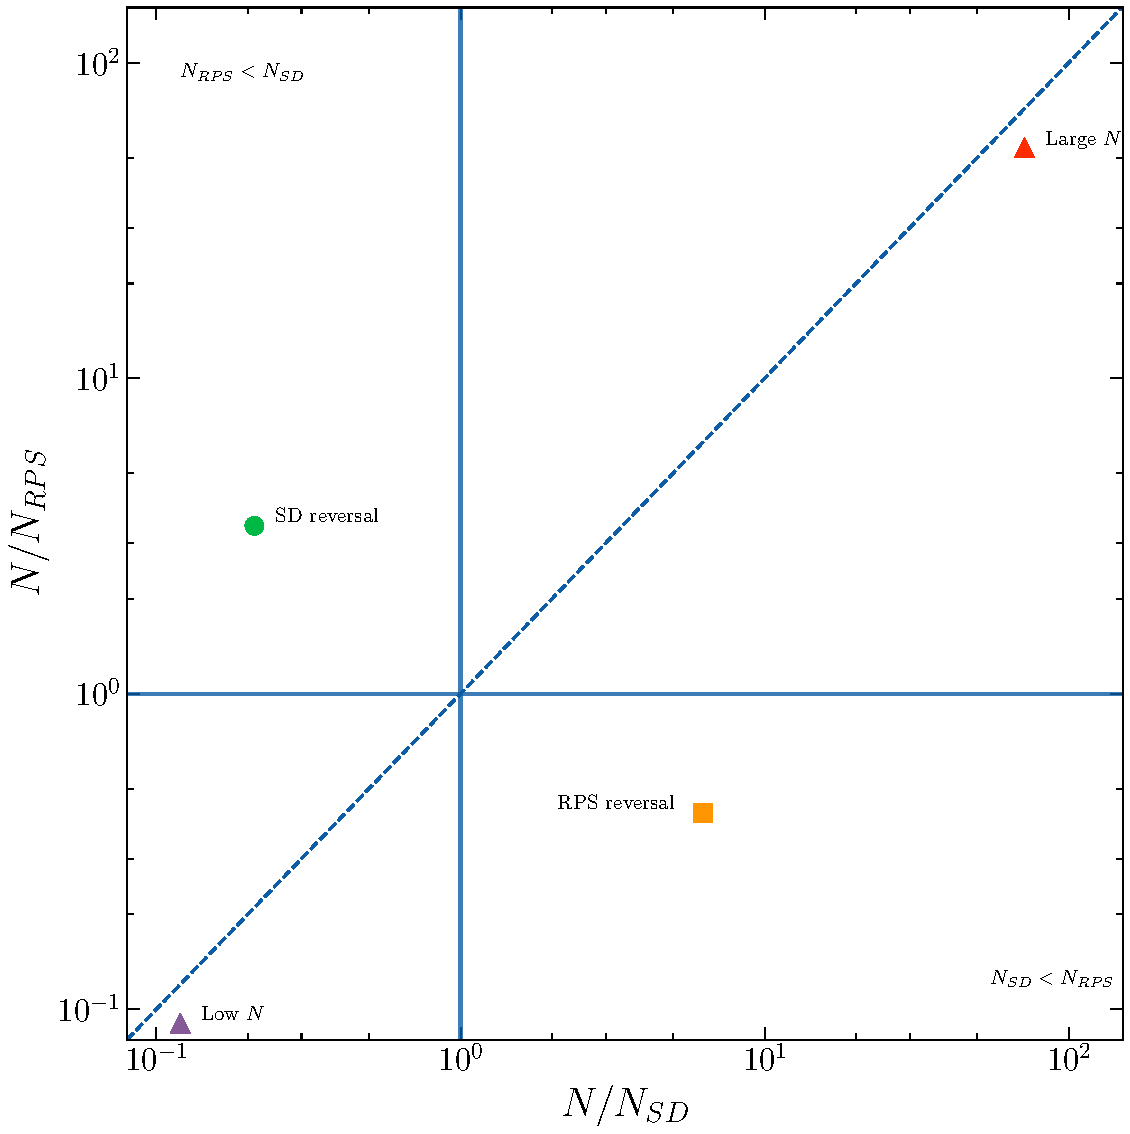
\includegraphics[width=1\textwidth]{./Figures/drift_cases/drift_shaded.pdf}};

  \begin{axis}[
    at={(img.south west)},
    anchor=south west,
    width=1\textwidth,
    height=1\textwidth*1, 
    xmin=0, xmax=4,         
    ymin=0, ymax=4,
    axis lines=none,          
    clip=false                 
  ]

    % Place the EPS thumbnails at data coordinates
    \node at (axis cs:1.2,3) {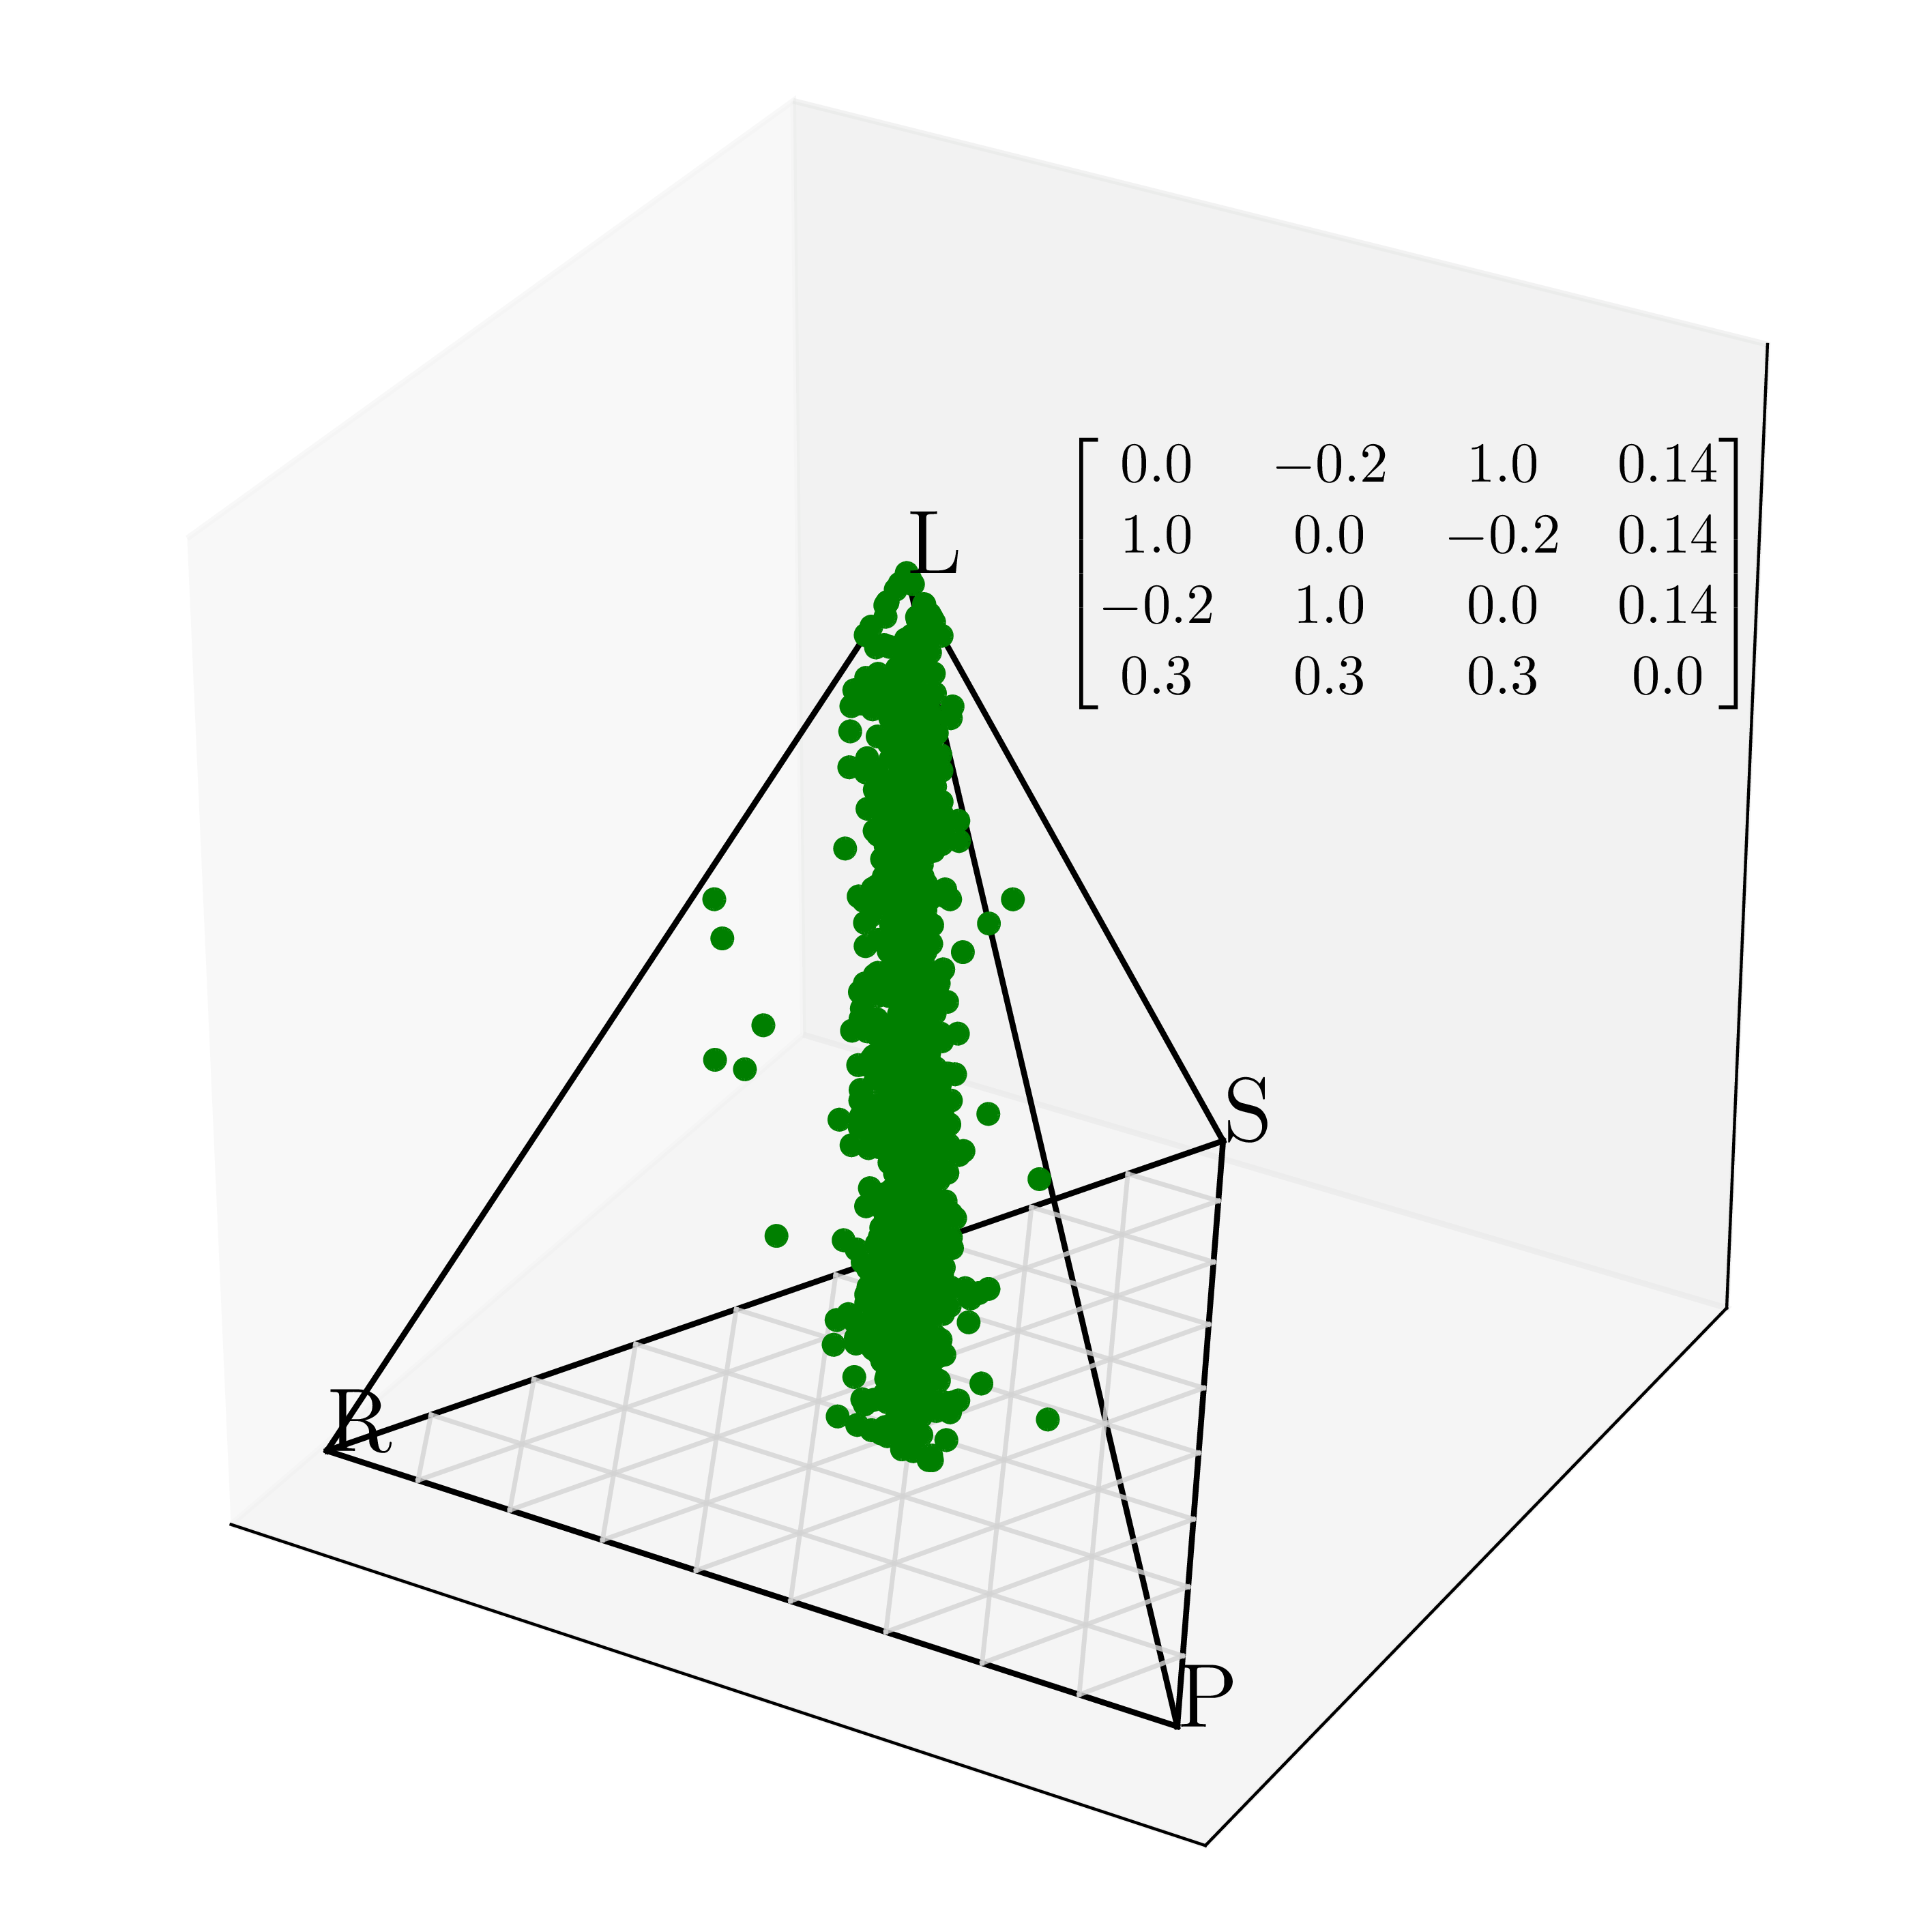
\includegraphics[width=5cm]{./Figures/drift_cases/rod_larger_inset.png}};
    \node at (axis cs:3.3,1) {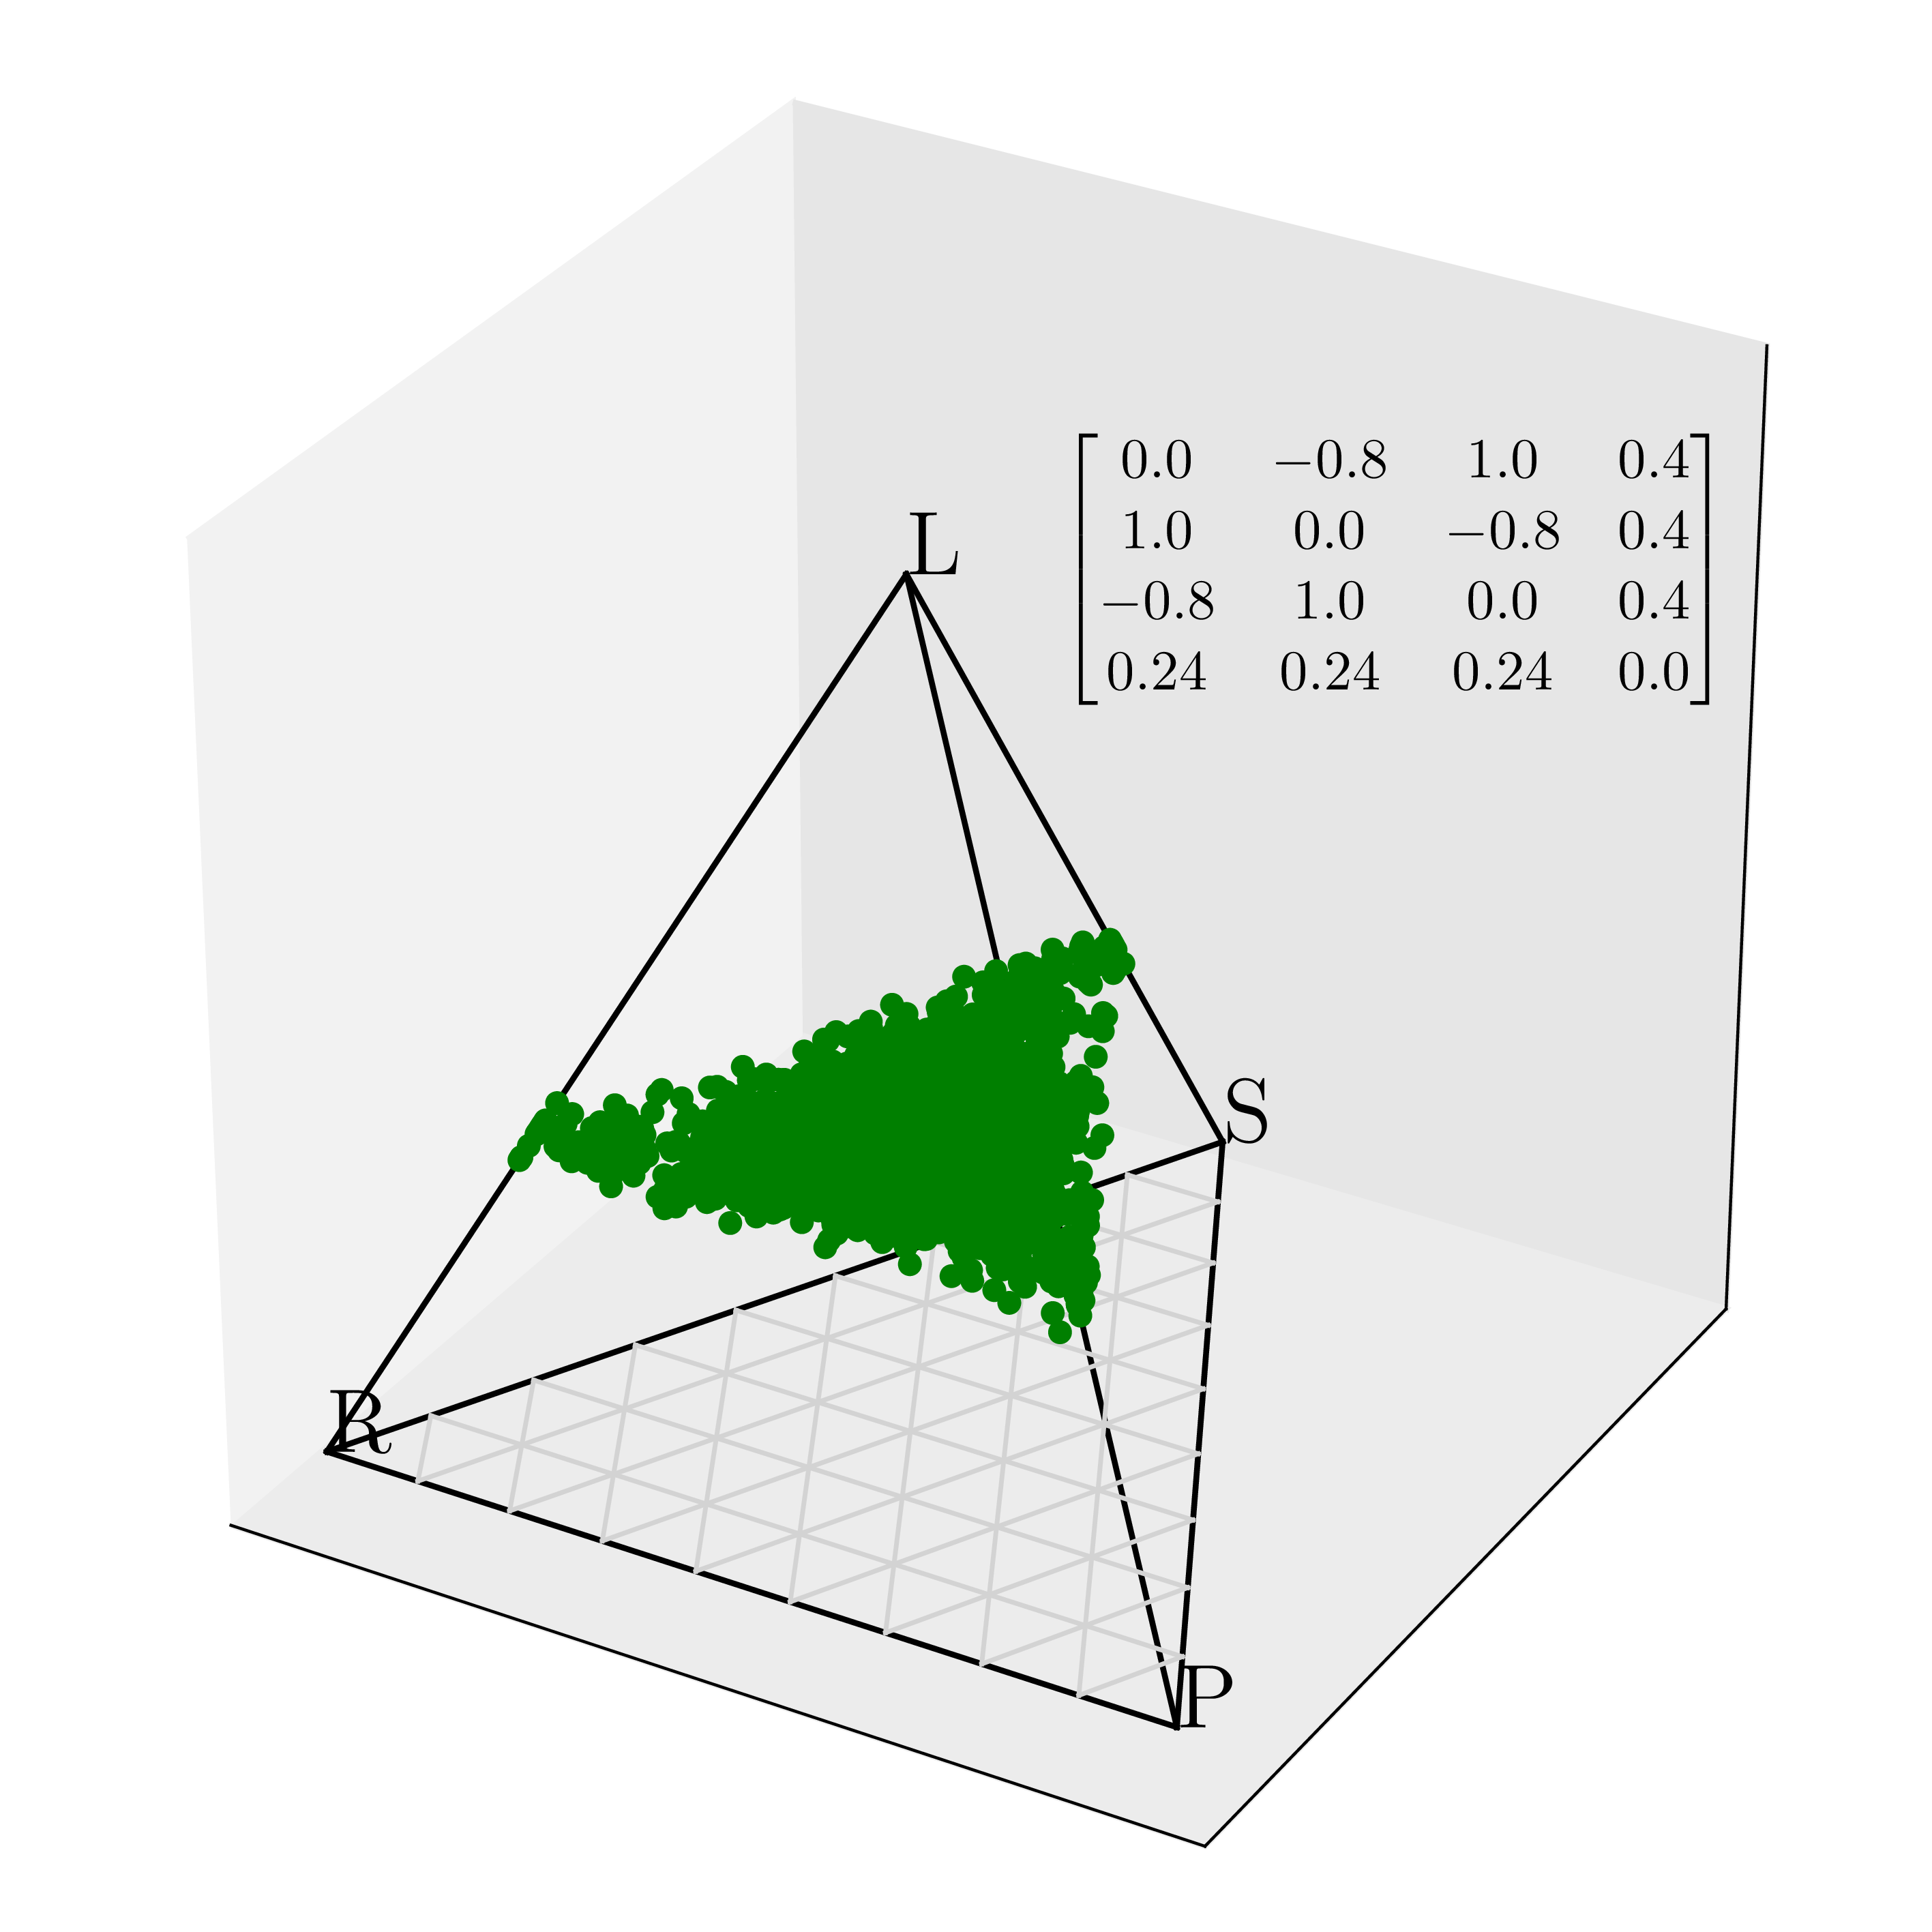
\includegraphics[width=5cm]{./Figures/drift_cases/disk_larger_inset.png}};
    \node at (axis cs:3.3,3.3) {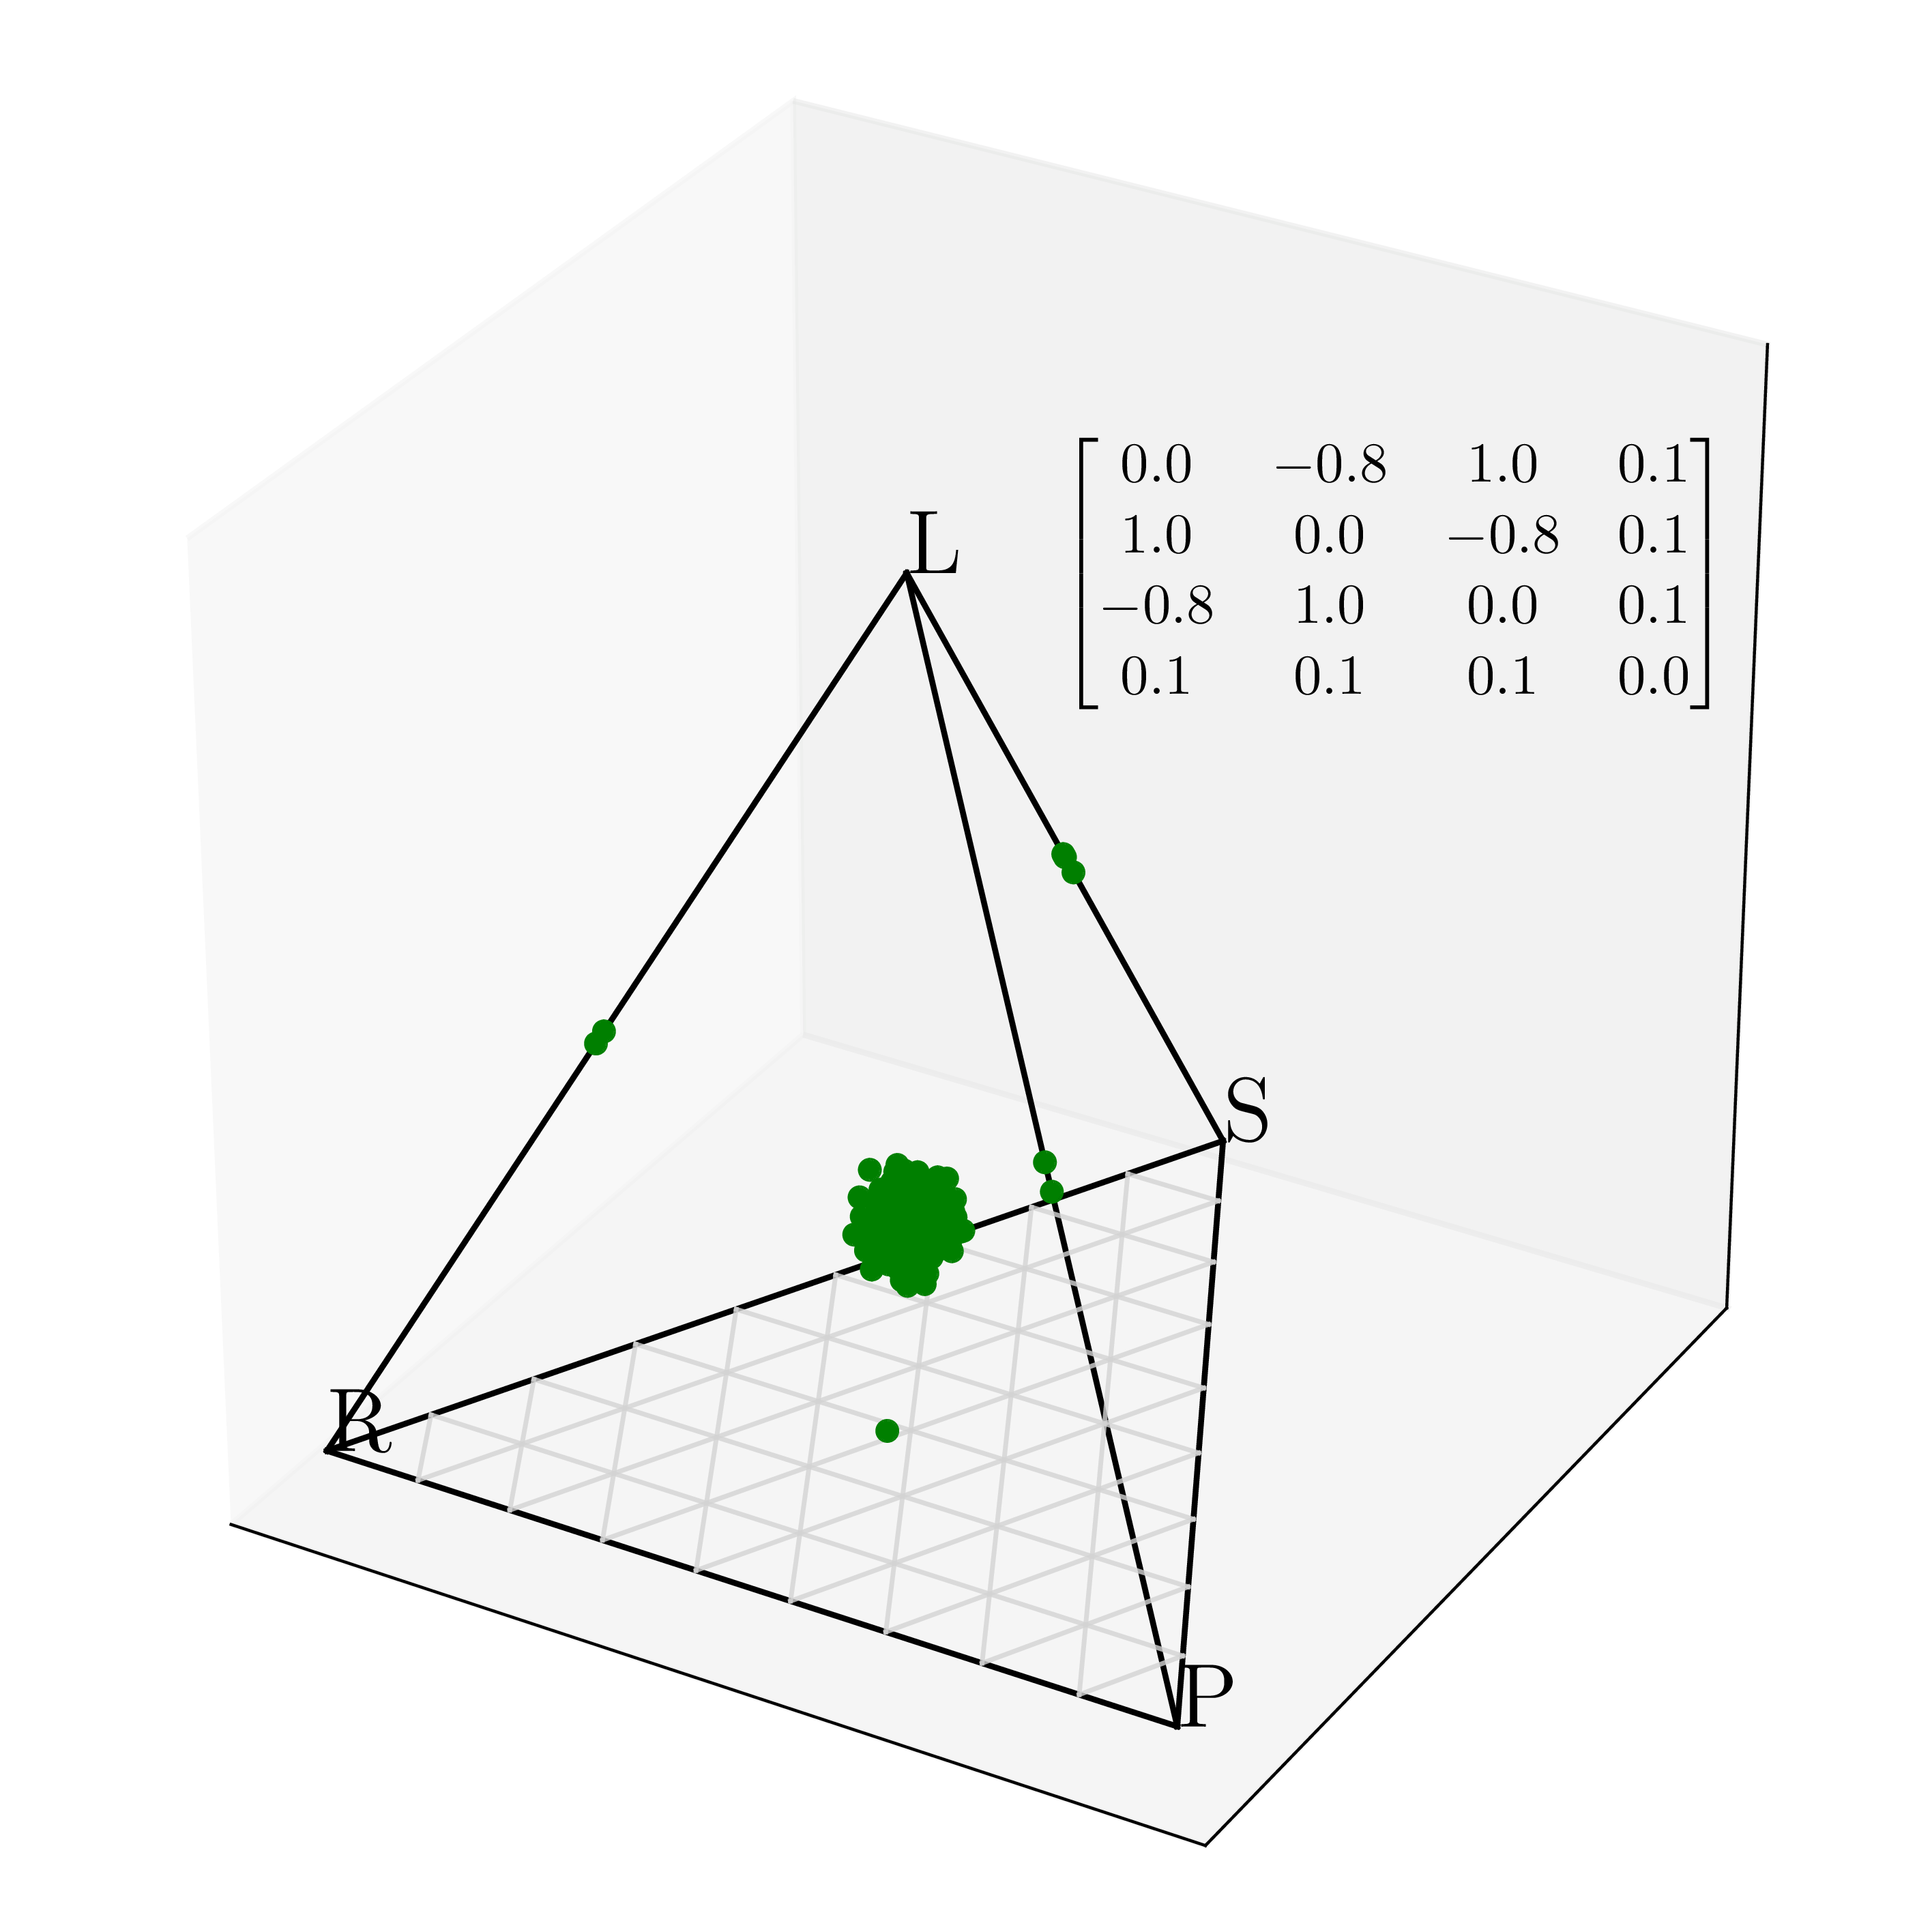
\includegraphics[width=5cm]{./Figures/drift_cases/large_N_inset.png}};
    \node at (axis cs:1.1,1.1) {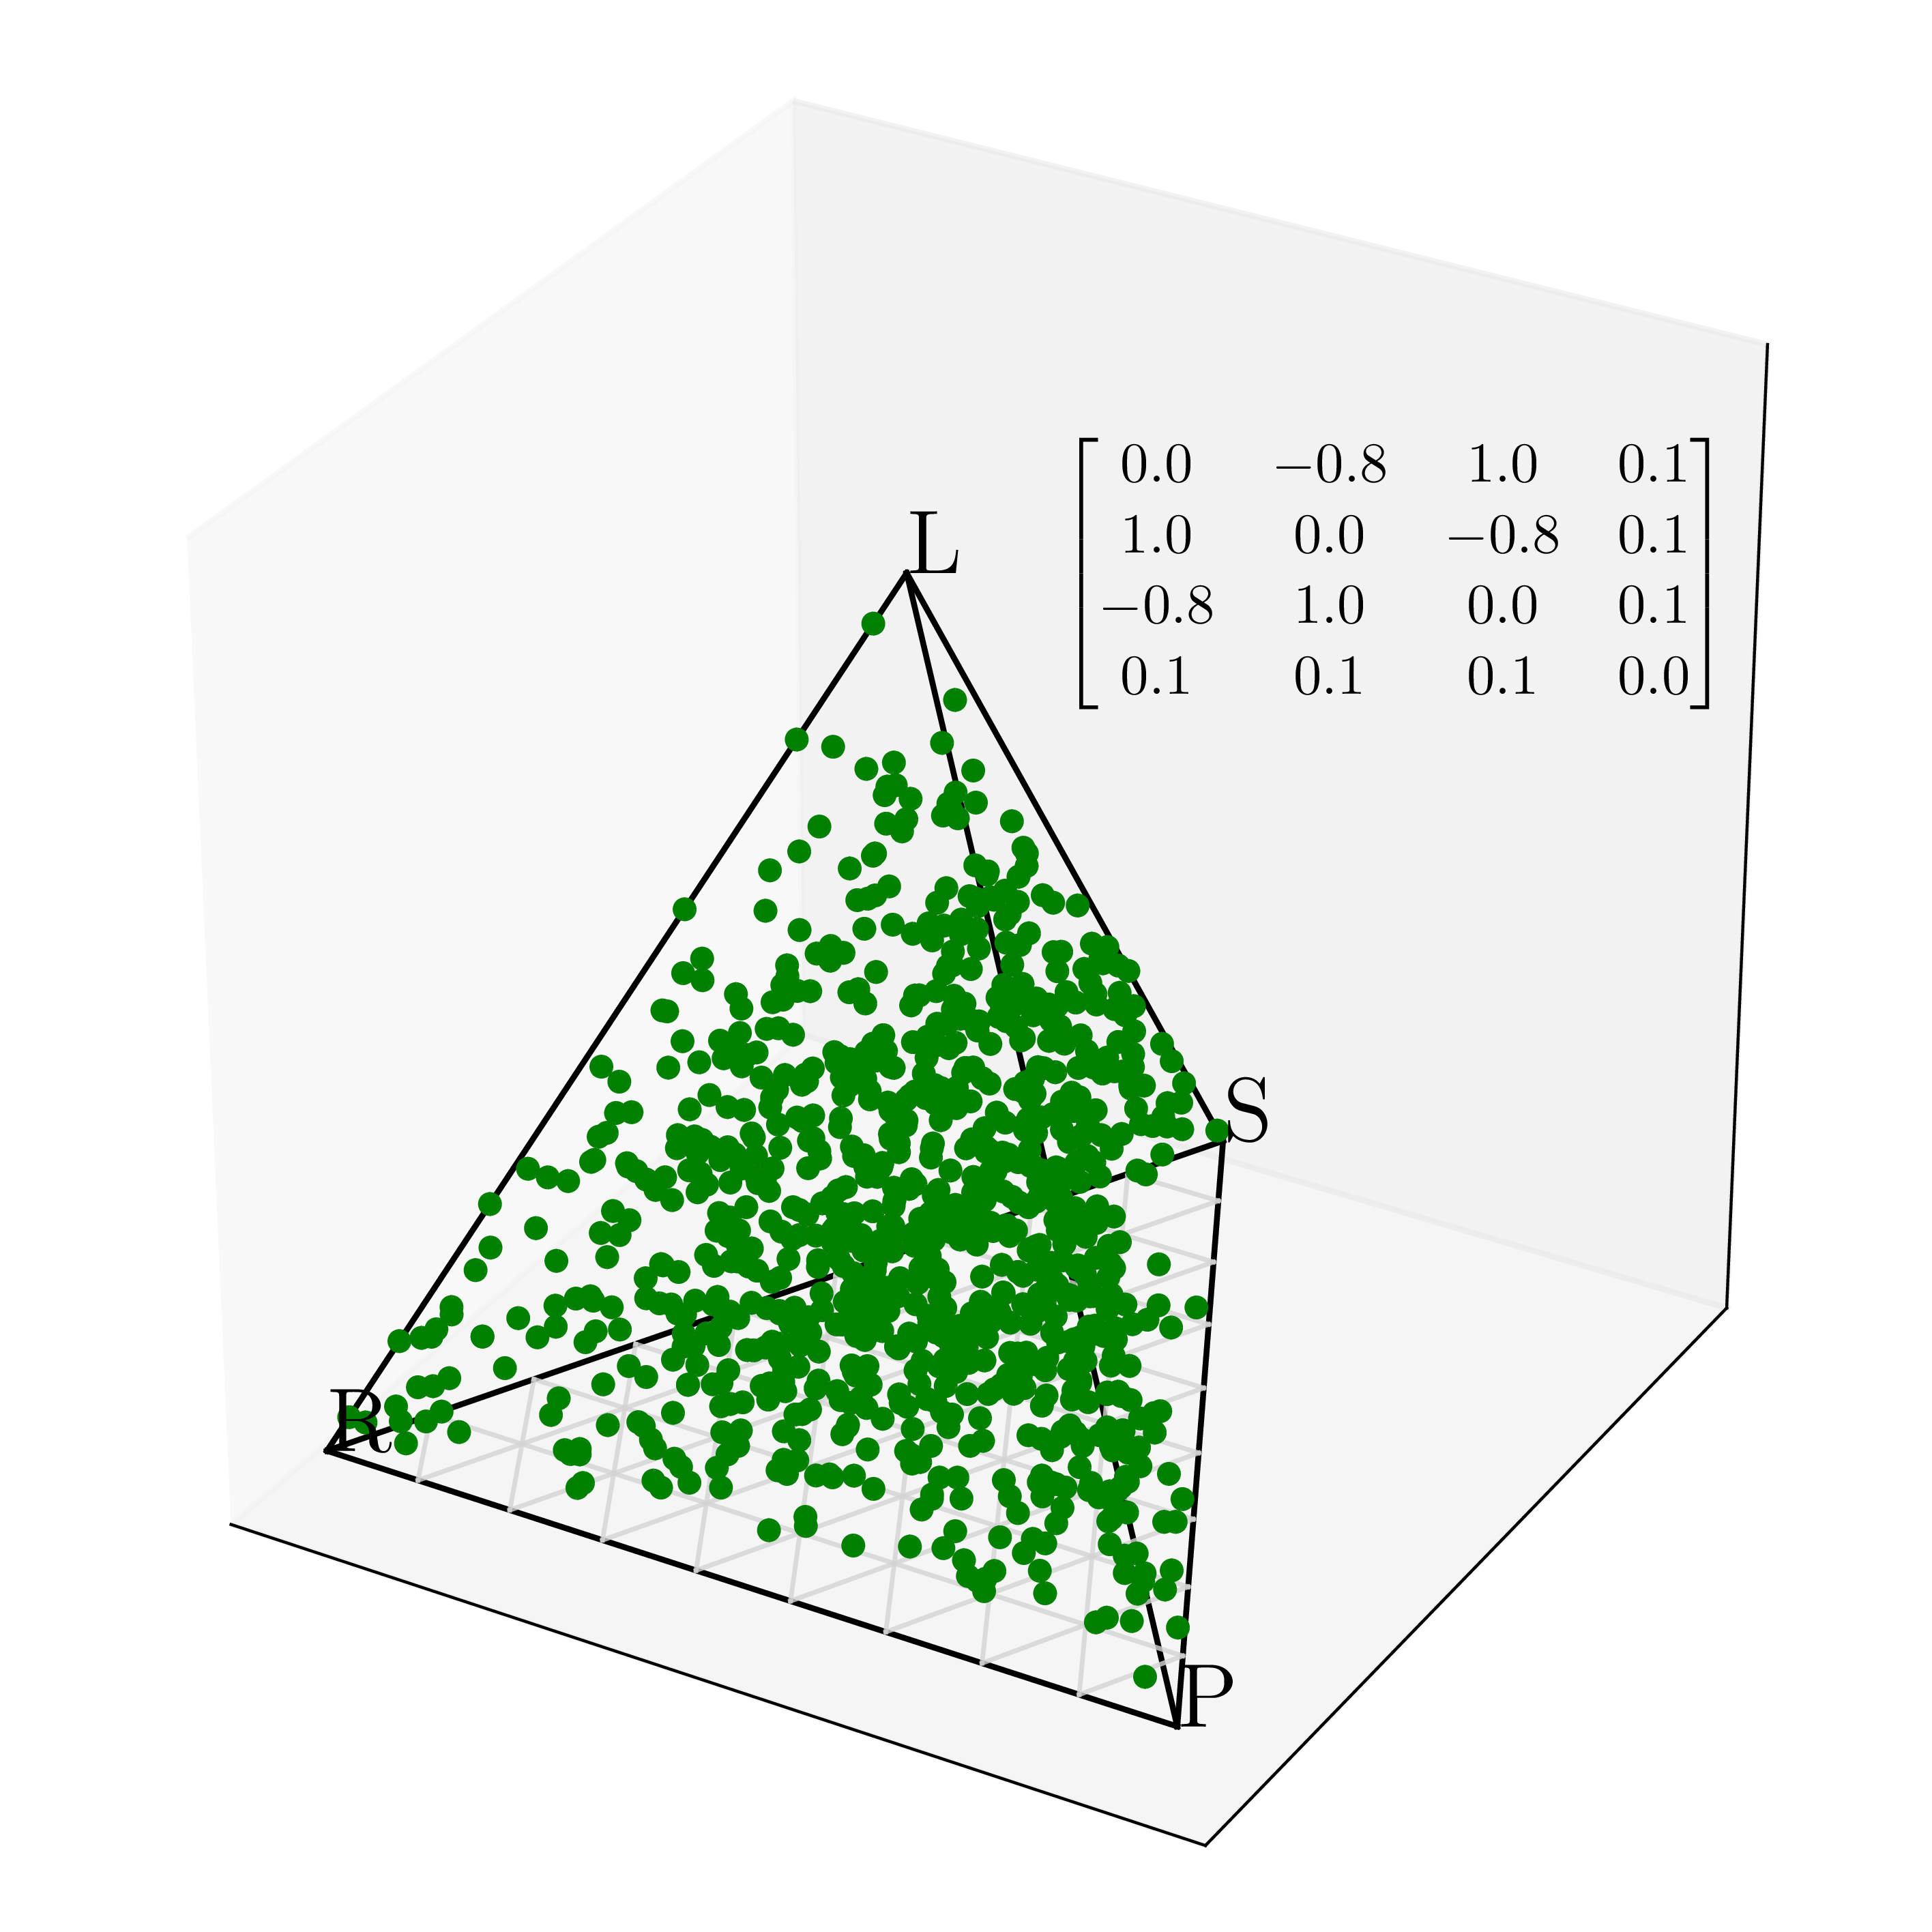
\includegraphics[width=5cm]{./Figures/drift_cases/low_pop_case_trans.png}};


  \end{axis}
\end{tikzpicture}
\caption{\label{drift_cases_fig} Comparison of the main drift reversal cases, notably the RPS and not SD reversal (disk like shape), SD and not RPS reversal (column shape), and 
large N Nash equilibrium stable case where $N >> N_c$ and chaotic low N case (drift in all directions)
 where $N << N_{RPS}, N << N_{SD}$. Each point corresponds to an independent trajectory which started from an initial 
 random point in the simplex.}
\end{figure*}



\section{Conclusion}
This project has analysed the evolutionary dynamics of a combined four-strategy game
combining a cyclic RPS structure and a snowdrift game, in infinite and 
finite populations under three different microscopic interaction processes.

In infinite populations a stable interior fixed point emerges in the combined game where all 
four strategies coexist under various different initial payoff matrices. Varying the 
RPS parameter $c$ changes the game from a neutrally stable orbit about the fixed point to an 
attracting fixed point within the RPS plane while trajectories also converge along the SD axis.

The main result of this project is that the combined game exhibits previous concepts of drift reversal, 
and that there are multiple distinct drift reversals in the system for each subgame. These have been shown 
to occur at two unique critical population sizes $N^\prime_{\mathrm{RPS}}$ and 
$N^\prime_{\mathrm{SD}}$ and for the local update process a closed form expression for these is derived.
These results are also computed numerically for the Moran process and the local fermi process through 
computation of the integrals and large-ensemble agent based simulations where they are approximated by one update step 
and averaged over many repeated simulations.

The relative ordering of the critical population sizes (if they both exist) and 
the actual population size $N$, determines four distinct
cases summarised in Fig.~\ref{drift_cases_fig}. When $N^\prime_{SD} < N < N^\prime_{RPS}$ drift reversal occurs 
in the RPS plane, when $N^\prime_{RPS} < N < N^\prime_{SD}$ the opposite is true and the reversal takes place in the 
vertical SD axis in the simplex. For very large population size the dynamics are correctly predicted by the 
deterministic replicator dynamics ($N \rightarrow \infty$) and for very low population size
there is a double drift reversal and the trajectories are absorbed by the boundaries, where the replicator 
dynamics predict a stable interior coexistence.

The microscopic update processes produce similar drift reversal behaviour in the combined game but with 
different trajectories and critical population sizes for identical initial parameters.
These become equivalent in the weak selection limit (neutral evolution) 
as the strength of selection $w \rightarrow 0$. Deterministic adjusted replicator dyanmics as 
the population size $N \rightarrow \infty$ are derived for each of the processes through a 
Kramers-Moyal expansion of the master equation resulting in a Fokker-Planck equation quantifying the effects
of drift and noise in the time evolution of the populations. The noise term has a factor of $1/N$ 
explaining the emergence of drift reversal in some cases when $N$ is small and the dynamics are 
qualitatively altered.

Some extensions that could be considered would be the inclusion of mutation where some strategies could randomly hop with 
a small probability to another. This would prevent boundary extinctions perhaps 
leading to clearer visualizations of some of the drift reversal cases at low populations, 
as for starting points near the edges of the faces of the simplex many trajectories immediately 
get absorbed through pure random noise. The mutation extension has and has been considered in
Ref.~\cite{general_moran_process} where the Moran and local update process with mutations is explored.

The analysis can also be extended to other combinations of $2 \times 2$ and 
$3 \times 3$ games and to higher-dimensional composite games
formed by embedding multiple payoff structures into a single larger matrix, combining a variety of
different dynamics. The number of drift observables can naturally be extended 
with one for each additional subgame
to fully characterise the stochastic dynamics in finite populations with more than two subgames.

\clearpage
\nocite{*}
\bibliographystyle{apsrev4-2}
\bibliography{report}

\end{document}
